\chapter[Persistent Homology for Amorphous Materials]{Persistent Homology for \\ Amorphous Materials}
\label{ch:ph}

\begin{chapterabstract}
Persistent homology is a technique in topological data analysis to find the fundamental topological features in a collection of points.
The applicability of persistent homology to the analysis of network materials is explored here for the relatively simple case of \td{} networks. 
XXXXX
\end{chapterabstract}

\section{Introduction to Persistent Homology}

The need for efficient methods to find structure in large and complex data sets is ever increasing in the age of ``big data''.
The field of topological data analysis (TDA) has emerged to address this need, driving the development of statistical tools to analyse and understand big, noisy, real\--world data \cite{Wasserman2018}.
One tool in particular has received significant attention, namely that of persistent homology \cite{Edelsbrunner2008}.
Persistent homology is concerned with finding the fundamental topological features of given set of points. 
In slightly plainer terms, here \textit{homology} means counting the number of connected components (``blobs'') and cycles (``holes'') in a system.
The persistence aspect arises from the fact that the these topological features can be calculated across different length scales, with those existing across multiple length scales being identified as more \textit{persistent}.
The more persistent a topological feature, the more it can be thought of as reflecting the true underlying system topology.

As with any new technique which arrives with much fanfare, persistent homology has been quickly appropriated for the study of chemical and physical systems.
In fact, the marriage of persistent homology and atomistic materials seems apt.
Atomic systems have long been thought of in terms of collections of point like particles, and the study of the emergent structure is deep\--rooted in the field.
Any process which can elucidate as yet hidden structure in materials, or improve its description naturally has potential to be extremely useful.
In this vein, research has already been conducted on applying persistent homology to diverse topics such as colloidal packings, porous media, water networks, fullerenes \cite{Carter2018,Robins2017,Jiang2018,Steinberg2019,Xia2015}, and of particular importance to this work, amorphous materials \cite{Hiraoka2016,Onodera2019,Nakamura2015,Gutierrez2019}.
Whilst these latter studies claim to highlight structures which are not available using more conventional techniques, quantify the medium range order in glasses, and explain phenomena such as the origin of the first sharp diffraction peak in disordered materials; the fact remains that persistent homology remains a qualitative descriptor, with some doubt as to what is the ``added value'' from this technique. 
In the words of Wassserman: ``\textit{...the main purpose of TDA is to help the data analyst summarize and visualize
complex datasets. Whether or not TDA can be used to make scientific discoveries is still unclear.}'' \cite{Wasserman2018}.

The purpose of this chapter is therefore to try and assess the utility of persistent homology in the context of \td{} amorphous materials, with the expectation that the interpretation may be simpler for these reduced dimensionality systems.
The conclusions drawn from this work may then bring insight to the analysis of three dimensional systems.
This chapter will begin by outlining the relevant theory to persistent homology, with the aid of small example systems.
Persistent homology will then be calculated for configurations of silica bilayers (from experiment and via triangle rafts), and subsequently generic random networks as produced from bond switching.

\section{Computing Persistent Homology}

This section will give a broad outline of the mathematical background behind persistent homology, but with the focus on a practicable implementation for studying physical \td{} networks.
It will begin by introducing the concept of a filtered simplicial complex, before discussing homology groups, persistent homology and the visualisation of persistence.
Actual numerical persistent homology calculations can be carried out with the Gudhi library \cite{gudhi}.

\subsection{Filtered Simplicial Complexes}

The input for a persistent homology calculation is simply a point cloud \ie{} a set of coordinates in Euclidean space.
\davidnote{change $\mathbf{r}$ in Voronoi chapter}.
\davidnote{change all $r_{ij}\rightarrow d_{ij}$}.
For materials, this corresponds to the set of atomic positions, $\mathbf{r}=\left\{r_1,r_2,\cdots,r_\mathcal{N}\right\}$, as obtained from simulation or for instance experimentally via STM.
%Two example point clouds are provided in figures \ref{fig:phexa} and \ref{fig:phexe}, corresponding to a crystalline and amorphous configuration respectively.
Using this point cloud, a filtered simplicial complex can be constructed \cite{Fugacci2016}.
To explain what is meant by a filtered simplicial complex, it is useful to break down this definition further:
\begin{itemize}
	\item An $m$\--simplex, $\sigma$, is a subset of the total points, $\sigma\subseteq\mathbf{r}$, with dimension $m=\abs{\sigma}-1$.
Put simply, a $0$\--simplex corresponds to a point, a $1$\--simplex to a line, a $2$\--simplex a triangle, a $3$\--simplex a tetrahedron, and so on.% and so forth.
	\item A simplicial complex, $\mathbf{K}$, is then a set of simplices, $\mathbf{K}=\left\{\sigma_1,\sigma_2,\dots\right\}$.
	\item A filtration of a simplicial complex, is a sequence of subcomplexes: $\mathbf{K}_a \subseteq \mathbf{K}_b \subseteq \cdots \subseteq \mathbf{K}$, where each subcomplex, $\mathbf{K}_\epsilon$, occurs at an increasing filtration value, denoted $\epsilon$ (see below).
\end{itemize}
For a given point cloud, there are many ways to then construct a filtered simplicial complex (Cech, Vietoris\--Rips, Witness \etc), each method identifying simplices and calculating filtration values in a different manner  \cite{Otter2017}.
In this thesis, for reasons which will become apparent, the \textit{alpha complex} is used.

As an illustration of these concepts, an introductory example with just three points is given in figure \ref{fig:phalpha}.
Considering only the simplices at first: figure \ref{fig:phalphaa} contains three 0\--simplices, the points $A$, $B$, $C$; figures \ref{fig:phalphab1} and \ref{fig:phalphab2} three 1\--simplices, the lines $AB$, $AC$, $BC$; figure \ref{fig:phalphac} a 2\--simplex, the triangle $ABC$.
Once the simplices have been identified, a filtration value, $\epsilon$, is computed and assigned to each.
For the alpha complex, filtration values are determined from the radius of the circumcircles containing the simplices.
The specific algorithm is as follows:
\begin{itemize}
	\item 0\--simplices: must have a filtration value of $\epsilon=0$.
	\item 1\--simplices: provided the circumcircle is empty, they have a filtration value equal to its radius, which for two points is equivalent to half the line length $\epsilon=d_{ij}/2$.
	If the circumcircle contains a 2\--simplex, then the filtration value is set to the filtration value of that simplex.
	\item 2\--simplices: have a filtration value equal to the circumradius of the three points.
\end{itemize}
These different cases are shown and explained in figure \ref{fig:phalpha}.

Having calculated the filtration values for each simplex, a subcomplex can be generated, $\mathbf{K}_\epsilon$, which contains only the simplices with filtration values less than or equal to $\epsilon$.
Finally, the filtered simplicial complex emerges as a sequence of subcomplexes at increasing filtration values from $\epsilon=0\rightarrow \infty$.
Again figure \ref{fig:phalpha} shows this process for the case of three points.
The first subcomplex, $\mathbf{K}_0$, will only consist of a set of discrete points (as in figure \ref{fig:phalphaa}).
As the filtration value increases, higher dimensionality simplices will be included, as lines and triangles form (as in figure \ref{fig:phalphab1}).
The last subcomplex, $\mathbf{K}_\infty$, will contain all the determined simplices (as in figure \ref{fig:phalphac}).
Crucially, for the alpha complex, this will be equivalent to the Delaunay triangulation.
This is the motivation for choosing the alpha complex, as the Delaunay triangulation (which has already appeared throughout this thesis as the dual of the Voronoi diagram), is well defined in two dimensions. 
As such it provides the best opportunity to relate the results of persistent homology to well understood systems.

\begin{figure}[tb]
	\centering
     
	\begin{subfigure}[b]{0.45\textwidth}
         \centering
         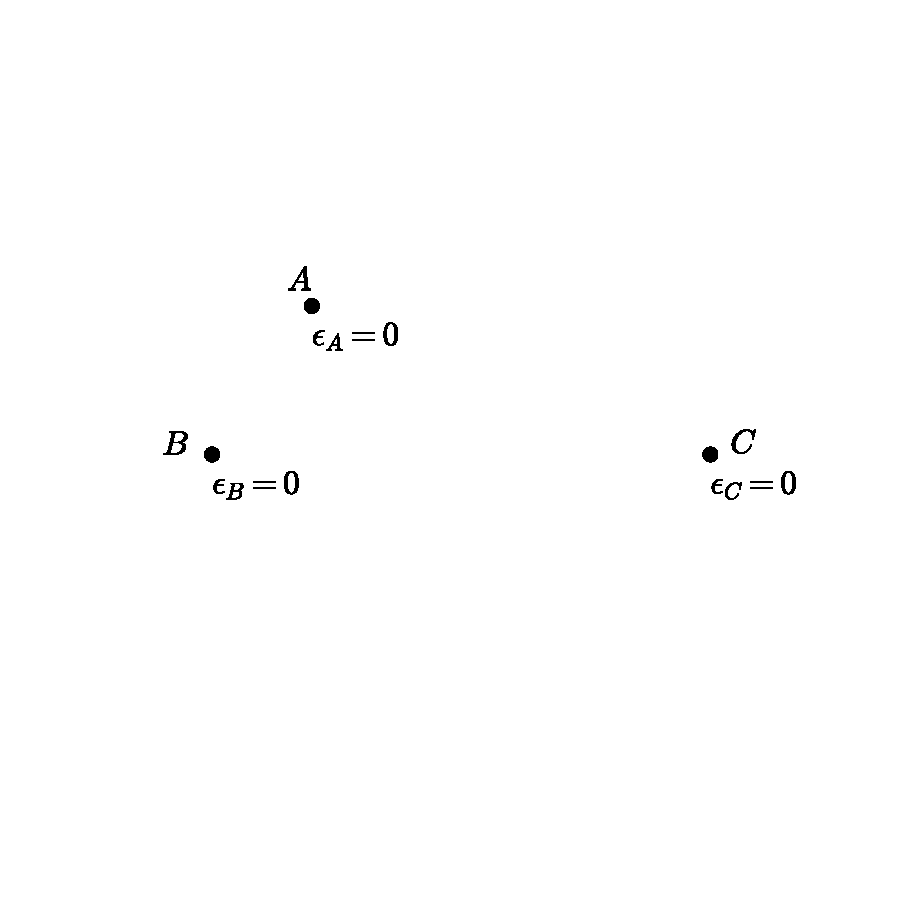
\includegraphics[width=\textwidth]{./figures/ph/alpha_a.pdf}
          \caption{$\sigma_1=\left\{A\right\}$, $\sigma_2=\left\{B\right\}$, $\sigma_3=\left\{C\right\}$; \\ $\mathbf{K}_0 = \left\{\sigma_1,\sigma_2,\sigma_3\right\}$}
         \label{fig:phalphaa}
     \end{subfigure}
     \hfill  
       \begin{subfigure}[b]{0.45\textwidth}
         \centering
         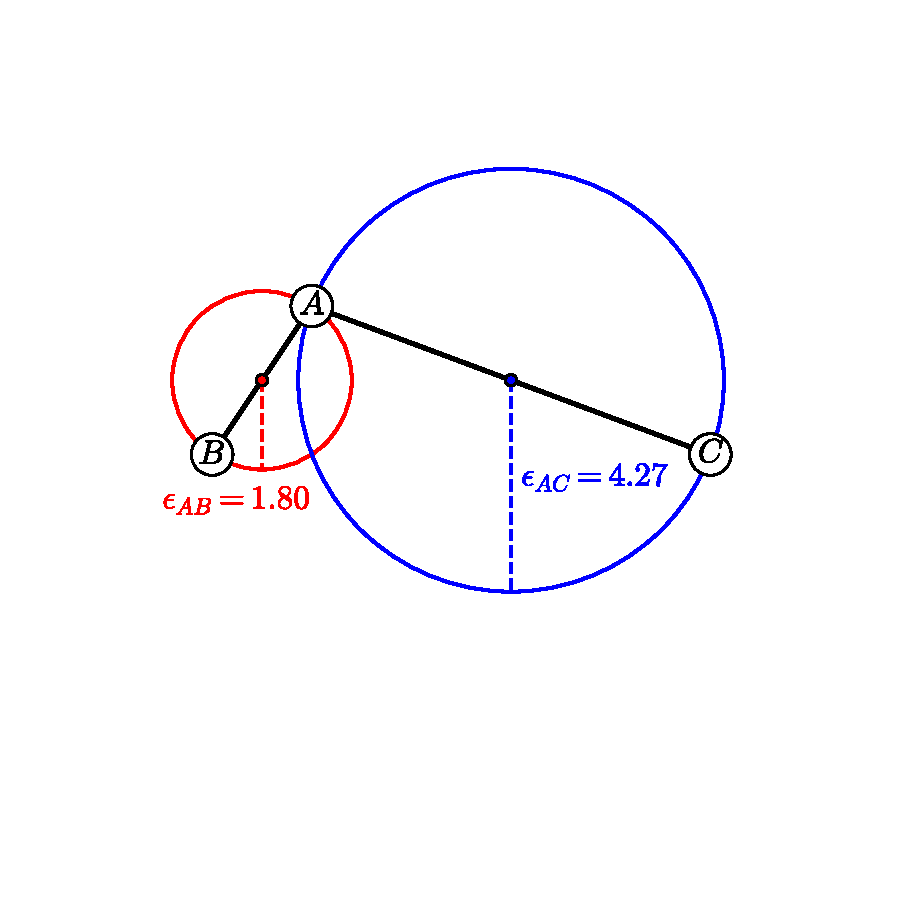
\includegraphics[width=\textwidth]{./figures/ph/alpha_b2.pdf}
        \caption{$\sigma_4=\left\{A,B\right\}$, $\sigma_5=\left\{A,C\right\}$; \\ $\mathbf{K}_{4.27} = \left\{\sigma_1,\sigma_2,\cdots,\sigma_5\right\}$}
         \label{fig:phalphab1}
     \end{subfigure}
     \hfill
        
      \vspace{0.5cm}
      \begin{subfigure}[b]{0.45\textwidth}
         \centering
         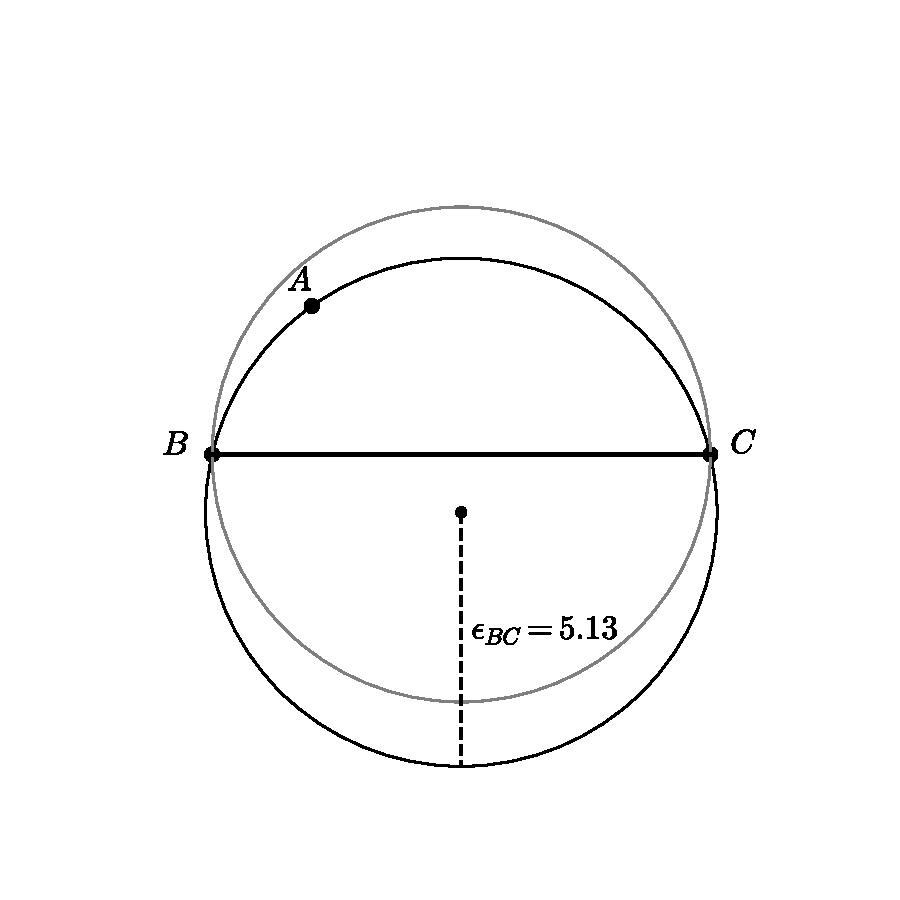
\includegraphics[width=\textwidth]{./figures/ph/alpha_b1.pdf}
         \caption{$\sigma_6=\left\{B,C\right\}$ \\ \phantom{x}}
         \label{fig:phalphab2}
     \end{subfigure}
     \hfill
      \begin{subfigure}[b]{0.45\textwidth}
         \centering
         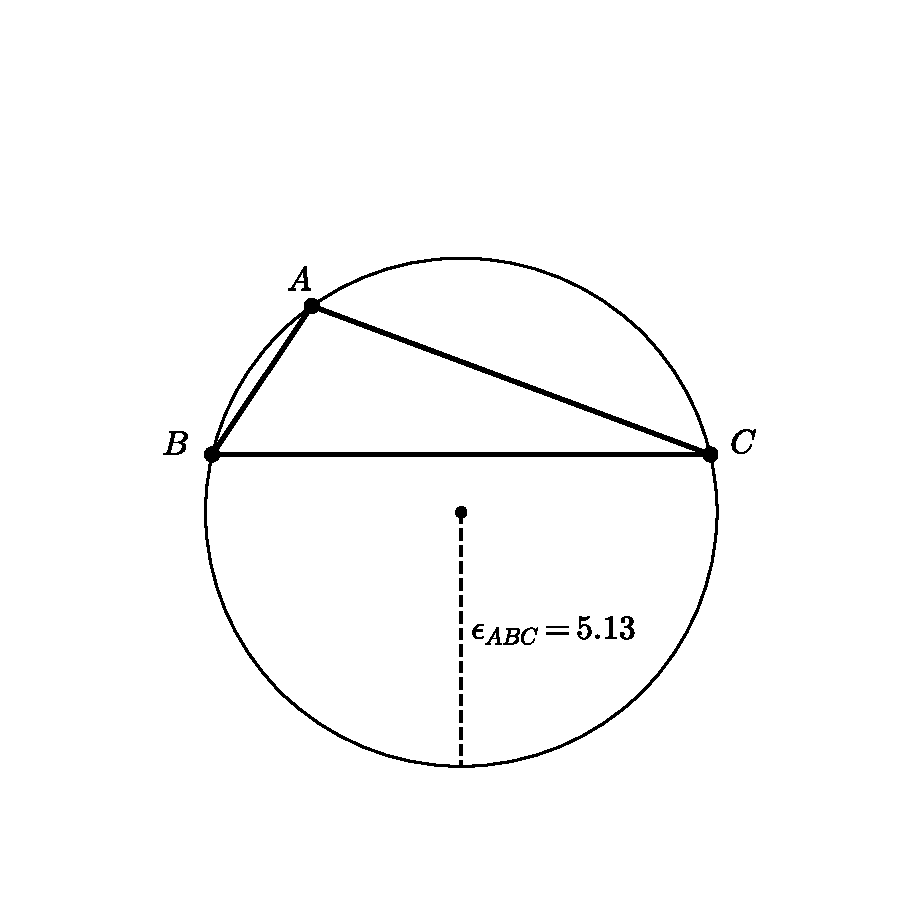
\includegraphics[width=\textwidth]{./figures/ph/alpha_c.pdf}
         \caption{$\sigma_7=\left\{A,B,C\right\}$; \\ $\mathbf{K}_{5.13}=\mathbf{K}_{\infty} = \left\{\sigma_1,\sigma_2,\cdots,\sigma_7\right\}$}
         \label{fig:phalphac}
     \end{subfigure}
     \hfill
    
	\caption{Construction of an alpha simplicial complex and its filtration. Panel (a) shows three 0\--simplices, with filtration values of $\epsilon=0$. Panel (b) shows an additional two 1\--simplices, with filtration values given by the radii of the respective circumcircles (dashed lines in black circles). Panel (c) shows an additional different 1\--simplex, in which the circumcircle (grey circle) contains the 3\--simplex $\left\{A,B,C\right\}$, and so the filtration value is set to the value of the 3\--simplex. Panel (d) shows an additional 3\--simplex with a filtration value given by the circumradius.
	These subfigures can also be viewed as a series of subcomplexes, as highlighted in the captions, with $\mathbf{K}_0\subseteq\mathbf{K}_{4.27}\subseteq\mathbf{K}_{5.13}=\mathbf{K}_\infty$. The final complex is the Delaunay triangulation of the original point set. Panel (c) is \textit{not} a subcomplex in the filtration, as it does not contain the simplices $\left\{A,B\right\}$, $\left\{A,C\right\}$, which have lower filtration values than $\left\{B,C\right\}$.}
	\label{fig:phalpha}
\end{figure}


\subsection{Homology and Persistent Homology}

Having introduced the notion of a filtered simplicial complex, the importance of homology and persistent homology can now be discussed.
To facilitate this, two more involved examples will be used.
Figures \ref{fig:phexa}\--\ref{fig:phexd} and \ref{fig:phexe}\--\ref{fig:phexh} show filtrations of alpha complexes for a crystalline and amorphous atomic configuration respectively, which will be referred to throughout this section.

In this context, homology is generally concerned with quantifying the number of $n$\--dimensional topological features in a simplicial complex.
For an alpha complex, these can either be 0\-- or 1\--dimensional.
The 0\--dimensional features correspond to the number of connected components, meaning the number of distinct groups of atoms.
The 1\--dimensional features are the number of ``cycles'' (or ``holes'') in the structure.
These are termed as such to differentiate from ``rings'' used elsewhere in this thesis, but often there will be significant overlap between the two.
Any alpha complex has the homology groups, $H_n\left(\mathbf{K}_\epsilon\right)$, which contain all the associated $n$\--dimensional features.
The rank of these groups are termed the Betti numbers, $\beta_n$ \cite{Zomorodian2005}.
To make this less abstract, one can see how this fits with the examples in figure \ref{fig:phex}:
\begin{itemize}
	\item Figures \ref{fig:phexa} and \ref{fig:phexe} have $\mathcal{N}=68$ and $\mathcal{N}=70$ individual points respectively, and so have Betti numbers of $\beta_0=\mathcal{N}$ and $\beta_1=0$.
	\item Figures \ref{fig:phexb} and \ref{fig:phexf} have all the atoms connected leading to the formation of $24$ cycles in both cases, and hence $\beta_0=1$ and $\beta_1=24$.
	\item Figures \ref{fig:phexc} and \ref{fig:phexg} both have a reduced number of cycles owing to the filtration values of triangular simplices being met. The Betti numbers are $\beta_0=1$, $\beta_1=12$ and $\beta_0=1$, $\beta_1=10$ in each case.
	\item Figures \ref{fig:phexd} and \ref{fig:phexh} have just one large connected component and no cycles, such that $\beta_0=1$ and $\beta_1=0$.
\end{itemize}
These examples illustrate a more general principle, that the ``starting point'', $\mathbf{K}_0$, will always have $\beta_0=\mathcal{N}$ and $\beta_1=0$, and the ``end point'', $\mathbf{K}_1$,  will always have $\beta_0=1$ and $\beta_1=0$ \ie{} trivial homology.
It is the filtration values in between which lead to richer behaviour.

This leads onto the notion of persistent homology.
Between any two subcomplexes at different filtration values, a selection of topological features will be common to both, whilst others will appear or disappear when moving from one to the other.
In other words, some features will \textit{persist} over the range of filtration values, whilst others will not.
To characterise this behaviour in the vocabulary of persistent homology, each feature is said to be ``born'' at a given filtration value, $b$, and ``die'' at a later value, $d$.
The lifetime, or persistence, of the feature is then quantified via $l=d-b$.
Finding and measuring the lifetimes of topological features is therefore the crux of persistent homology.
In the first instance, it is the longest lived features which are normally of most interest, as these are considered to be representative of the true system topology.
In the case of \td{} atomic materials, this ought to be reflective of the ring structure.
However, other more fleeting features can also be useful, as these intermediate features act as signatures for some medium range ordering \cite{Nakamura2015,Onodera2019}. 

\begin{figure}[tb]
	\centering
     
      \begin{subfigure}[b]{0.22\textwidth}
         \centering
         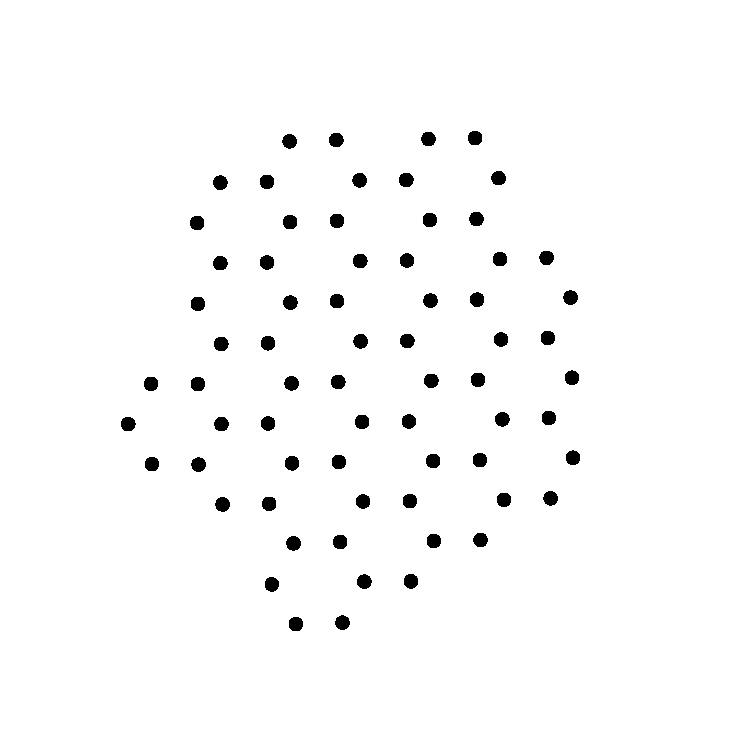
\includegraphics[width=\textwidth]{./figures/ph/ph_ex_crys_0.pdf}
         \caption{$\mathbf{K}_0$,\\ $\beta_0=68$, $\beta_1=0$}
         \label{fig:phexa}
     \end{subfigure}
     \hfill
      \begin{subfigure}[b]{0.22\textwidth}
         \centering
         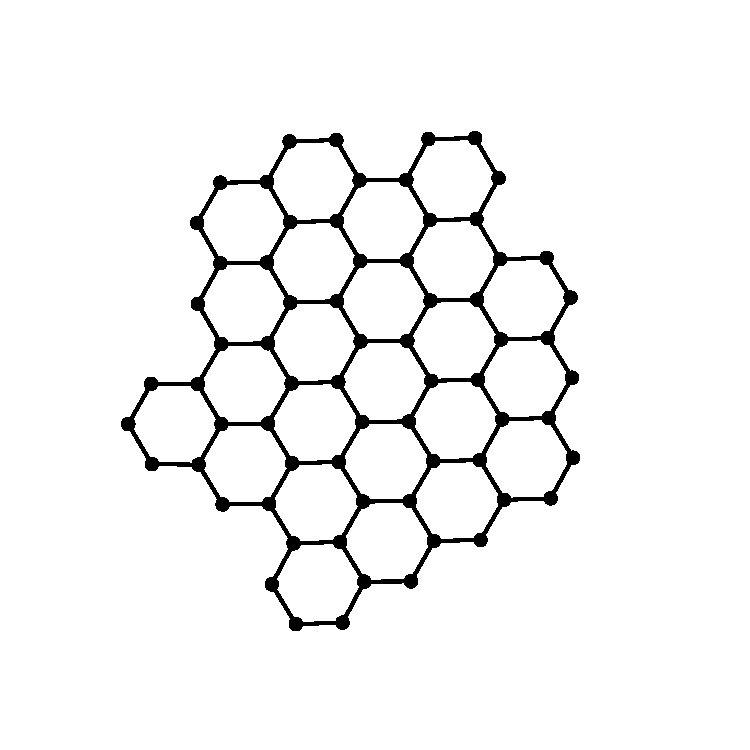
\includegraphics[width=\textwidth]{./figures/ph/ph_ex_crys_12.pdf}
         \caption{$\mathbf{K}_{0.55}$,\\ $\beta_0=1$, $\beta_1=24$}
         \label{fig:phexb}
     \end{subfigure}
     \hfill
     \begin{subfigure}[b]{0.22\textwidth}
         \centering
         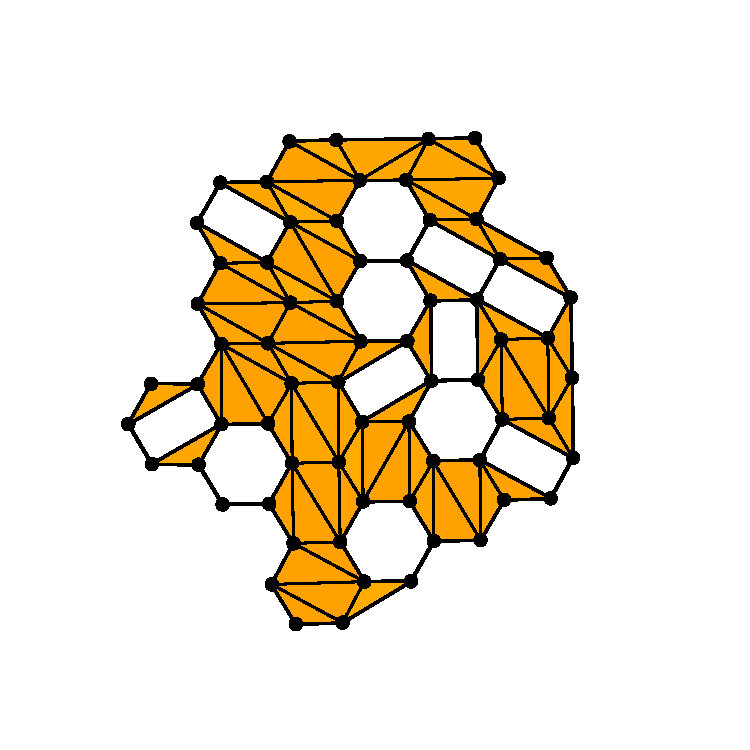
\includegraphics[width=\textwidth]{./figures/ph/ph_ex_crys_20.pdf}
         \caption{$\mathbf{K}_{0.99}$,\\ $\beta_0=1$, $\beta_1=12$}
         \label{fig:phexc}
     \end{subfigure}
     \hfill
     \begin{subfigure}[b]{0.22\textwidth}
         \centering
         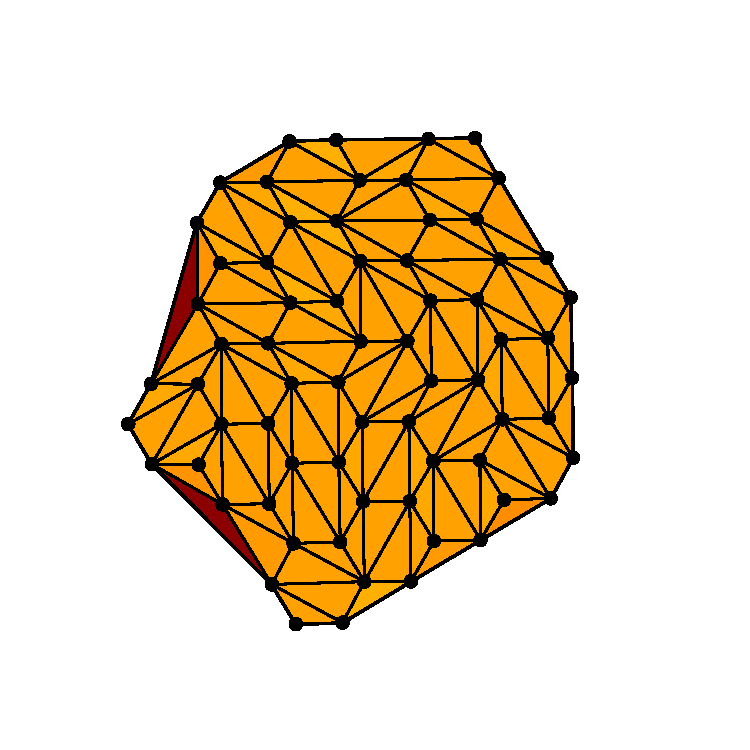
\includegraphics[width=\textwidth]{./figures/ph/ph_ex_crys_inf.pdf}
         \caption{$\mathbf{K}_\infty$,\\ $\beta_0=1$, $\beta_1=0$}
         \label{fig:phexd}
     \end{subfigure}
     
     \vspace{0.5cm}
     \begin{subfigure}[b]{0.22\textwidth}
         \centering
         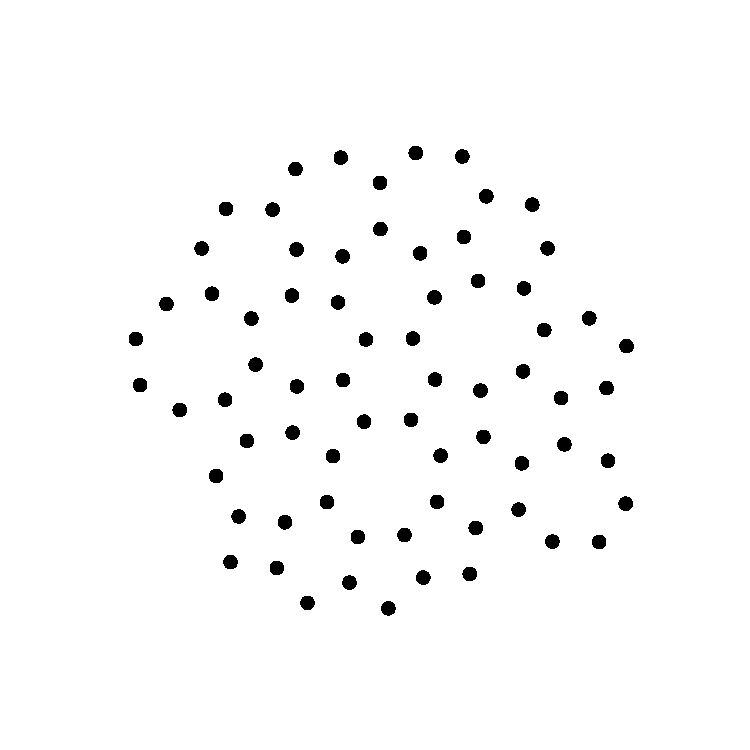
\includegraphics[width=\textwidth]{./figures/ph/ph_ex_amorph_0.pdf}
         \caption{$\mathbf{K}_0$,\\ $\beta_0=70$, $\beta_1=0$}
         \label{fig:phexe}
     \end{subfigure}
     \hfill
      \begin{subfigure}[b]{0.22\textwidth}
         \centering
         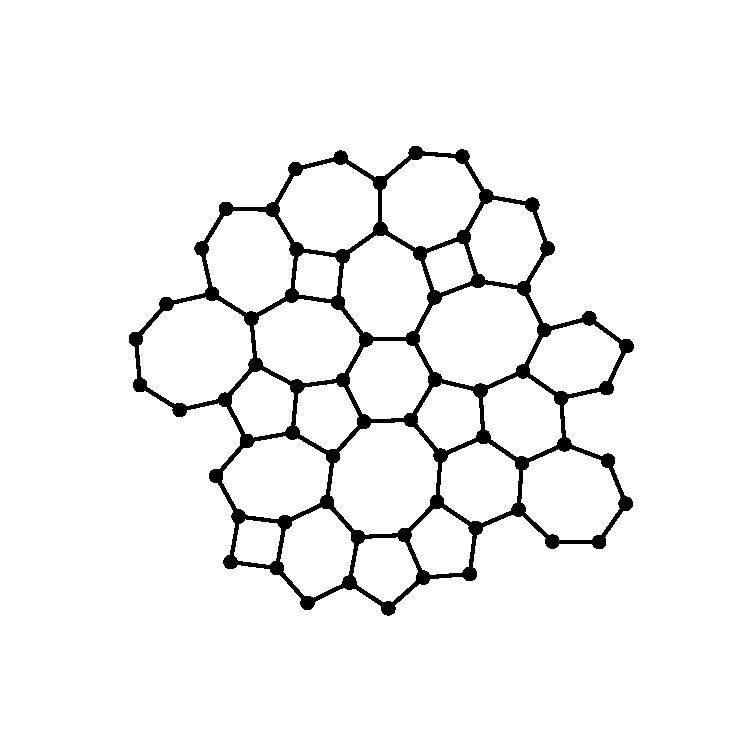
\includegraphics[width=\textwidth]{./figures/ph/ph_ex_amorph_12.pdf}
         \caption{$\mathbf{K}_{0.55}$,\\ $\beta_0=1$, $\beta_1=24$}
         \label{fig:phexf}
     \end{subfigure}
       \hfill
      \begin{subfigure}[b]{0.22\textwidth}
         \centering
         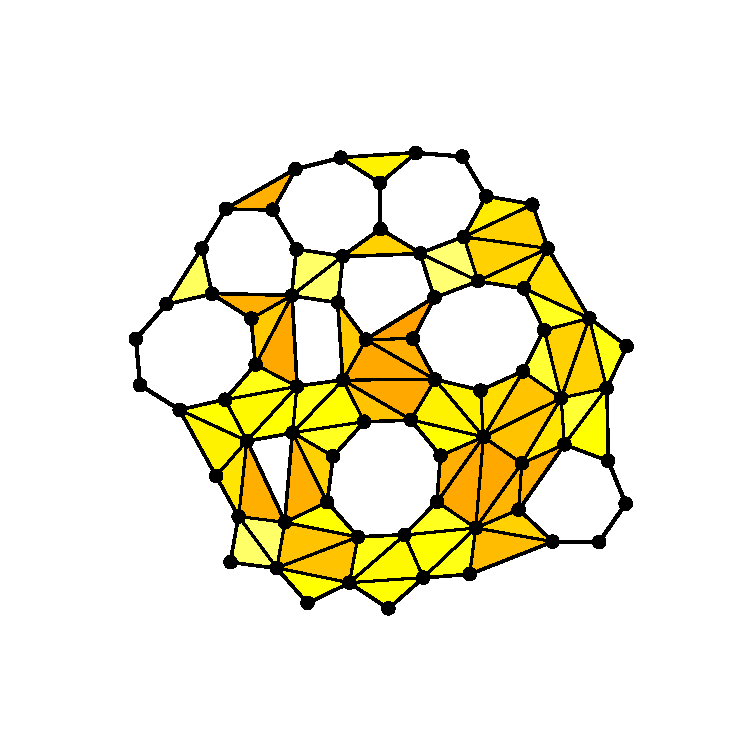
\includegraphics[width=\textwidth]{./figures/ph/ph_ex_amorph_20.pdf}
         \caption{$\mathbf{K}_{0.99}$,\\ $\beta_0=1$, $\beta_1=10$}
         \label{fig:phexg}
     \end{subfigure}
       \hfill
      \begin{subfigure}[b]{0.22\textwidth}
         \centering
         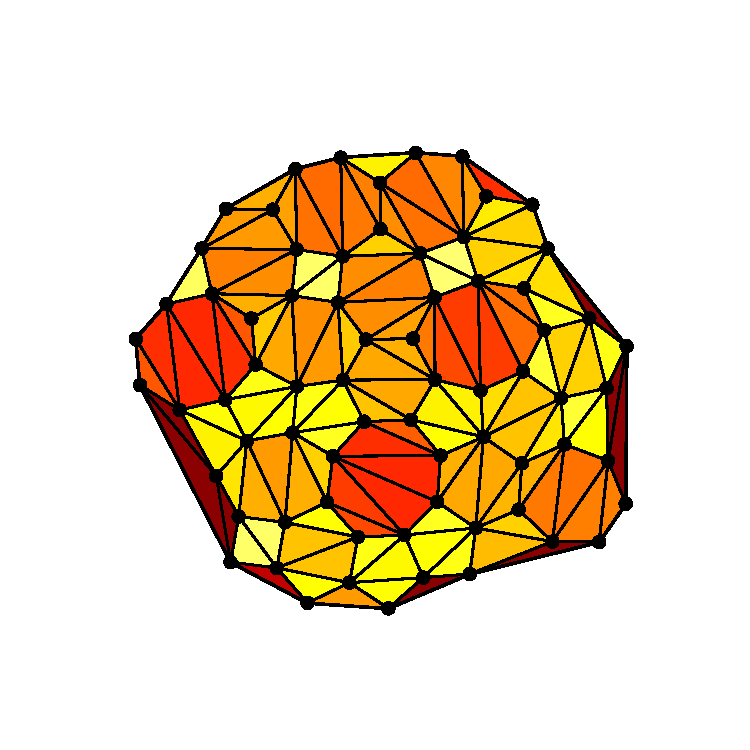
\includegraphics[width=\textwidth]{./figures/ph/ph_ex_amorph_inf.pdf}
         \caption{$\mathbf{K}_\infty$,\\ $\beta_0=1$, $\beta_1=0$}
         \label{fig:phexh}
     \end{subfigure}
   
	\caption{Filtered alpha complexes for a crystalline (a)\--(d) and amorphous (e)\--(h) configurations. The Betti numbers for the 0\-- and 1\--dimensional features are also given in the captions, corresponding to the number of connected components and cycles respectively. In addition 2\--simplices are coloured according to their filtration value, with yellow$\rightarrow$red indicating a larger filtration value. This highlights that all 2\--simplices form almost simultaneously in the crystalline case, resulting in the death of all cycles, whilst in the amorphous case the formation is more gradual such that larger cycles tend to persist longer.}
	\label{fig:phex}
\end{figure}

\subsection{Visualising Persistence}

After running a persistent homology calculation by generating a filtered simplicial complex, finding the topological features and determining the lifetimes of each, the results still have to be presented in a way that highlights the fundamental features and facilitates extraction of the key topological properties of the system.
There are multiple ways to do this, some of which are more suitable for small systems and some for large aggregated datasets.
These are outlined below, with examples given in figure \ref{fig:exvis}, in reference to the small crystalline and amorphous configurations discussed in figure \ref{fig:phex}.
\begin{itemize}
	\item \textbf{Persistence barcode}: represents the lifetime of each topological feature as a bar, starting at the birth value and terminating at the death value (see figures \ref{fig:exvisa}, \ref{fig:exvisb}). The barcode therefore contains all information about each feature, and whilst useful for small samples, it becomes difficult to interpret when there are a large number of features. In addition short lived features are difficult to identify.
	
	\item \textbf{Evolution in Betti numbers}: plots the total number of each $n$\--dimensional feature for each filtration value (see figures \ref{fig:exvisc}, \ref{fig:exvisd}), and so provides more coarse\--grained information than the barcode. It is equivalent to counting the number of bars at a specific filtration value.
	
	\item \textbf{Persistence diagram}: plots the birth and death values of each feature as a scatter diagram (see figures \ref{fig:exvise}, \ref{fig:exvisf}). This gives a more holistic view of the data as a whole. For large data sets, histogramming can be used, with points coloured by their relative multiplicities. The persistence diagram is therefore suitable for visualising large amounts of aggregate information.
	
%	\item \textbf{Lifetime distribution function}: presents a histogram of the lifetimes of each feature. This is useful for analysing a large number of features, but loses information on the exact birth and death values.
\end{itemize}
For all these visualisation methods, it is worth emphasising that the filtration value, $\epsilon$, has units of length, and so is normally quoted in terms of the equilibrium bond length, $r_0$. 

Although these visualisation methods have been introduced here, they will be interpreted only at a very high level, with more detailed analysis provided in the analysis sections.
Examining the results for the two example systems in \ref{fig:exvis}, one can see that the crystalline and amorphous systems have both similarities and differences.
To begin with, the 0\--dimensional features appear very similar across all plots, with $b=0$ and $d=r_0/2$.
This is because in atomic systems, the average bond length is highly restricted, and so all atoms become connected in a very small range of filtration values, corresponding to half the mean bond length (as the filtration value measures the circumradius of the 1\--simplex).
As such the $0$\--dimensional features provide little insight for atomic systems, and will be neglected in the analysis in this chapter.

On the other hand, the 1\--dimensional features show significant differences between the crystalline and amorphous configurations.
Both systems have 24 persistent bars in their barcode (figures \ref{fig:exvisa}, \ref{fig:exvisb}), which are born at $b=\epsilon=r_0/2$, but the lifetimes vary considerably. 
For the crystalline system, all persistent cycles (corresponding to hexagons) terminate at almost the same value of $\epsilon=r_0$, whereas in the amorphous case there is a much broader distribution of values.
These values will be discussed in detail in section \davidnote{link}, but as might be expected, it is related to the radius of the circumcircle into which each polygon is inscribed. 
It is not only the persistent cycles which show variation though.
The persistence diagrams, figures \ref{fig:exvise} and \ref{fig:exvisf}), also show that the short lived features, which lie close to the line $b=d$, show greater variation in the amorphous case.
This will also be explored in greater depth in the remainder of the chapter.

What these small examples serve to demonstrate, is that persistent homology does show some promise for capturing the disorder in amorphous materials.
The question is whether these visualisations can be systematically interpreted to quantify this disorder, and obtain information which is not available via alternative methods.

\begin{figure}[tbp]
	\centering
     
      \begin{subfigure}[b]{0.45\textwidth}
         \centering
         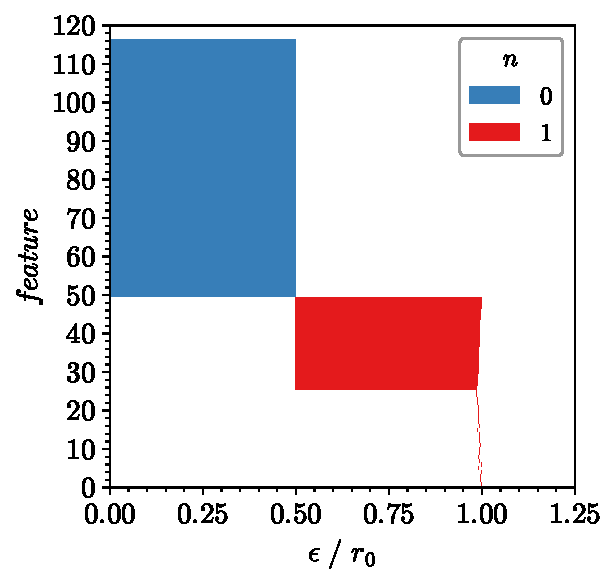
\includegraphics[width=\textwidth]{./figures/ph/ex_c_barcode.pdf}
         \caption{}
         \label{fig:exvisa}
     \end{subfigure}
     \hfill
     \begin{subfigure}[b]{0.45\textwidth}
         \centering
         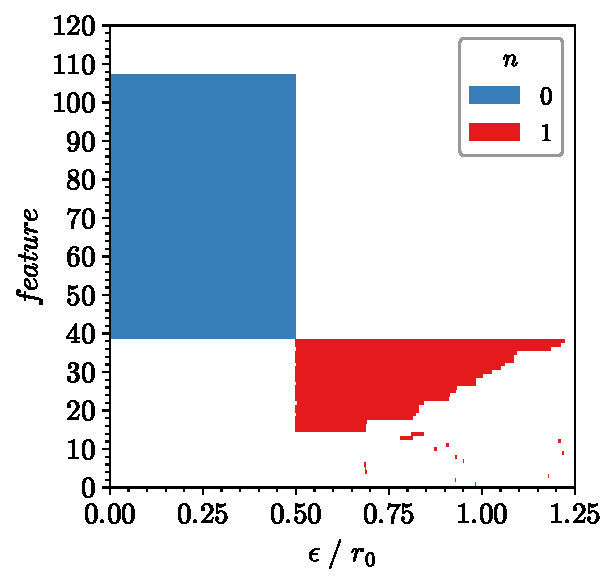
\includegraphics[width=\textwidth]{./figures/ph/ex_a_barcode.pdf}
         \caption{}
         \label{fig:exvisb}
     \end{subfigure}
     \hfill
     
     \begin{subfigure}[b]{0.45\textwidth}
         \centering
         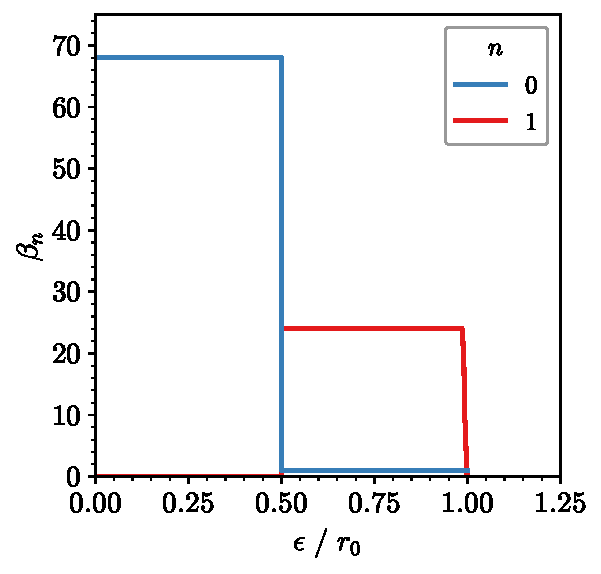
\includegraphics[width=\textwidth]{./figures/ph/ex_c_betti.pdf}
         \caption{}
         \label{fig:exvisc}
     \end{subfigure}
     \hfill
     \begin{subfigure}[b]{0.45\textwidth}
         \centering
         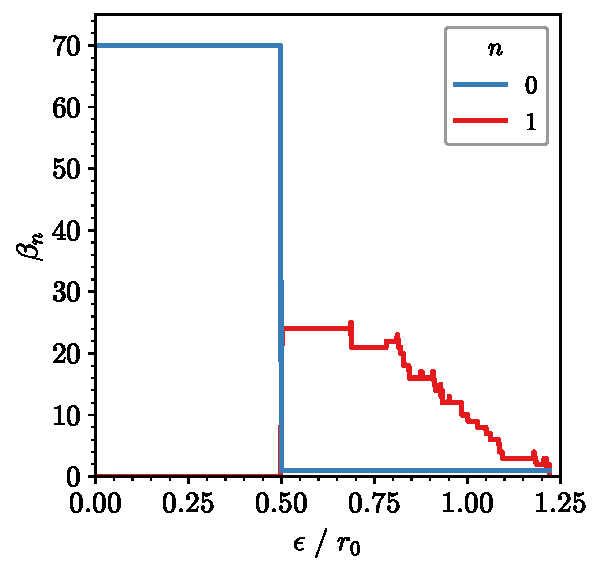
\includegraphics[width=\textwidth]{./figures/ph/ex_a_betti.pdf}
         \caption{}
         \label{fig:exvisd}
     \end{subfigure}
     \hfill
     
     \begin{subfigure}[b]{0.45\textwidth}
         \centering
         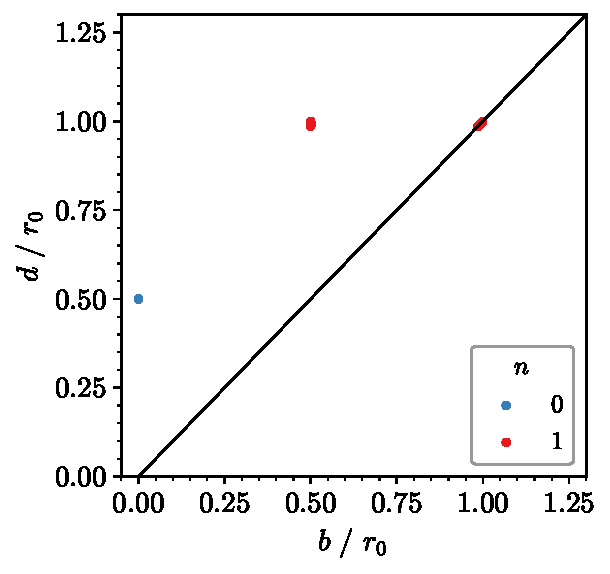
\includegraphics[width=\textwidth]{./figures/ph/ex_c_pd.pdf}
         \caption{}
         \label{fig:exvise}
     \end{subfigure}
     \hfill
     \begin{subfigure}[b]{0.45\textwidth}
         \centering
         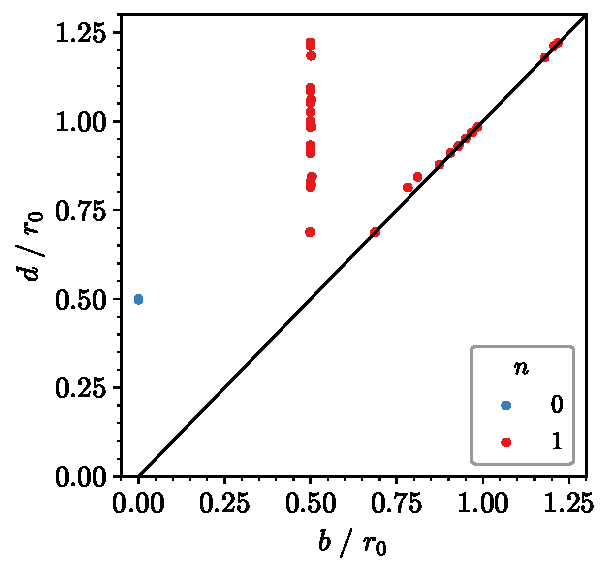
\includegraphics[width=\textwidth]{./figures/ph/ex_a_pd.pdf}
         \caption{}
         \label{fig:exvisf}
     \end{subfigure}
     \hfill
    
	\caption{Different methods for visualising results of persistence of topological features. The left column gives results for the example crystalline configuration in figure \ref{fig:phex}, and the right column the amorphous configuration in the same figure. Panels (a), (b) show the persistence barcode, panels (c), (d) the evolution in Betti numbers with filtration value and (e), (f) the persistence diagram.}
	\label{fig:exvis}
\end{figure}

\section{Persistent Homology with Triangle Rafts}

\begin{figure}[tb]
	\centering
     
      \begin{subfigure}[b]{0.48\textwidth}
         \centering
         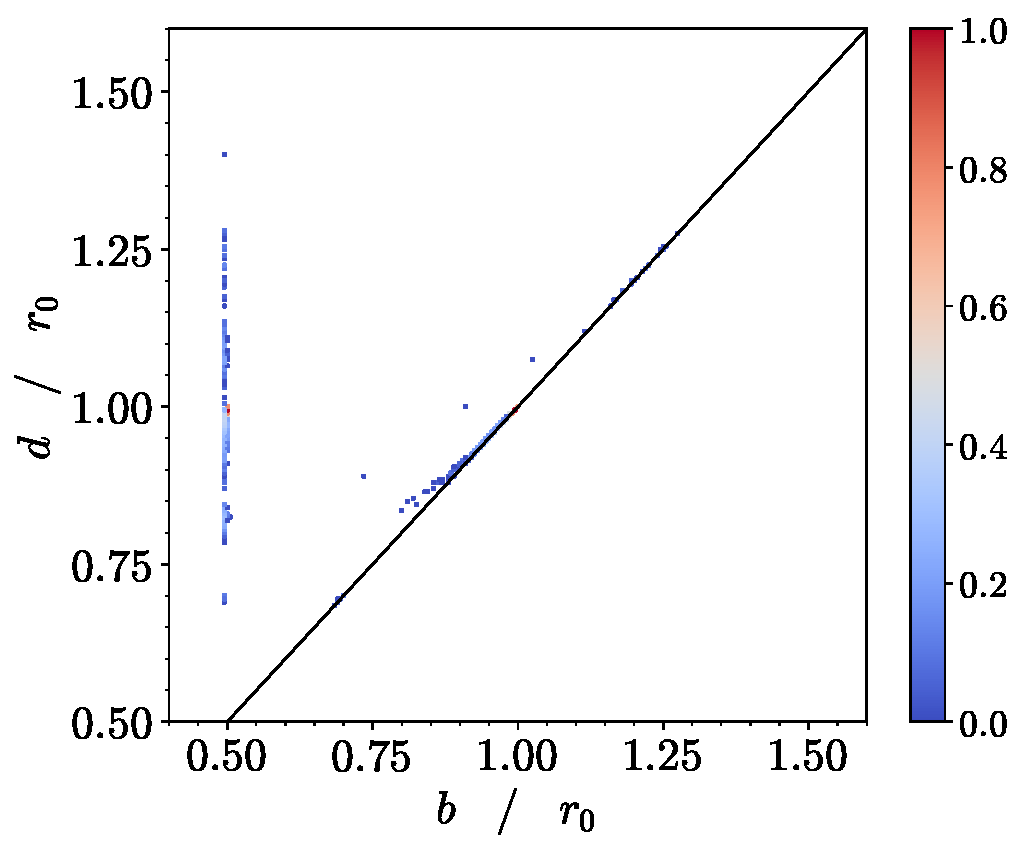
\includegraphics[width=\textwidth]{./figures/ph/t-4500_tr_pd.pdf}
         \caption{}
         \label{fig:trpda}
     \end{subfigure}
     \hfill
      \begin{subfigure}[b]{0.48\textwidth}
         \centering
         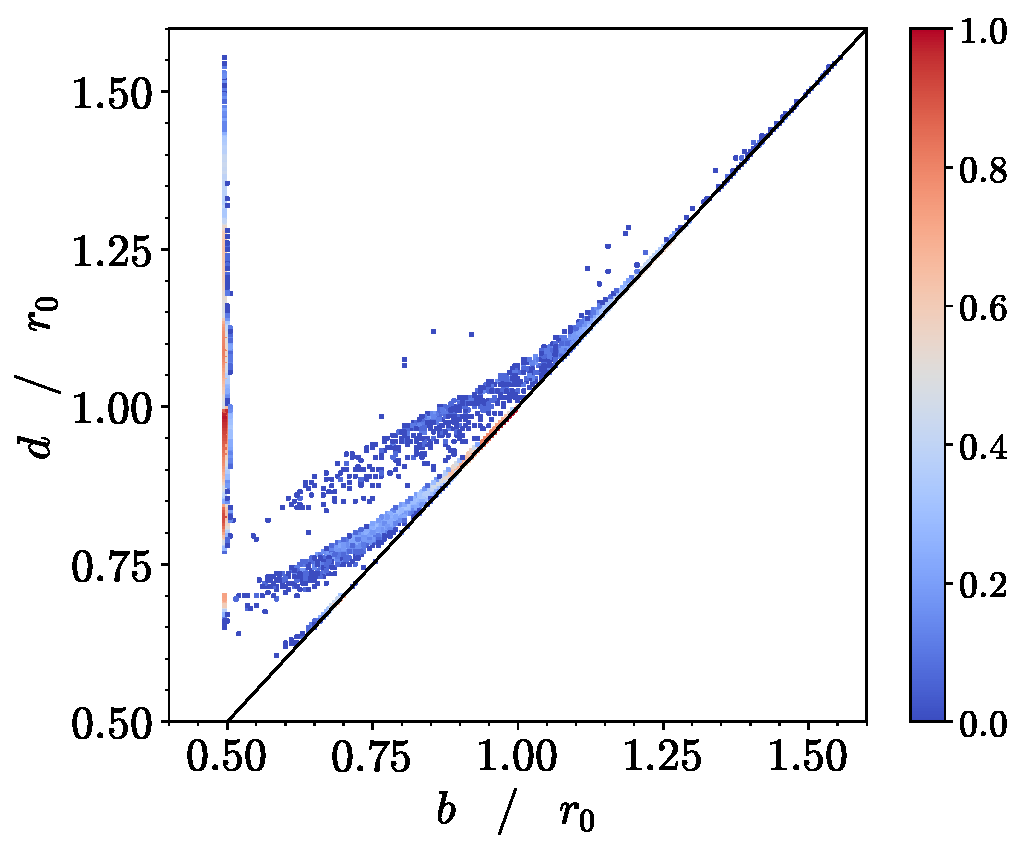
\includegraphics[width=\textwidth]{./figures/ph/t-3600_tr_pd.pdf}
         \caption{}
         \label{fig:trpdb}
     \end{subfigure}
     \hfill
     
     \begin{subfigure}[b]{0.48\textwidth}
         \centering
         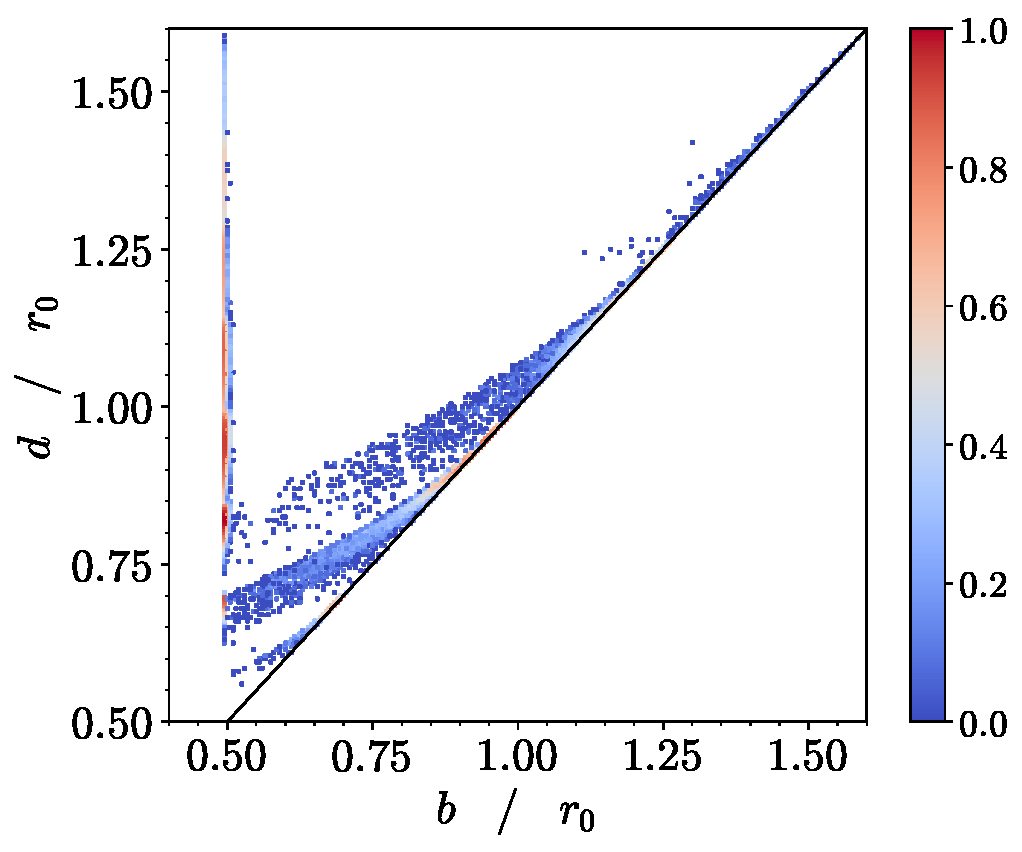
\includegraphics[width=\textwidth]{./figures/ph/t-2700_tr_pd.pdf}
         \caption{}
         \label{fig:trpdc}
     \end{subfigure}
     \hfill
      \begin{subfigure}[b]{0.48\textwidth}
         \centering
         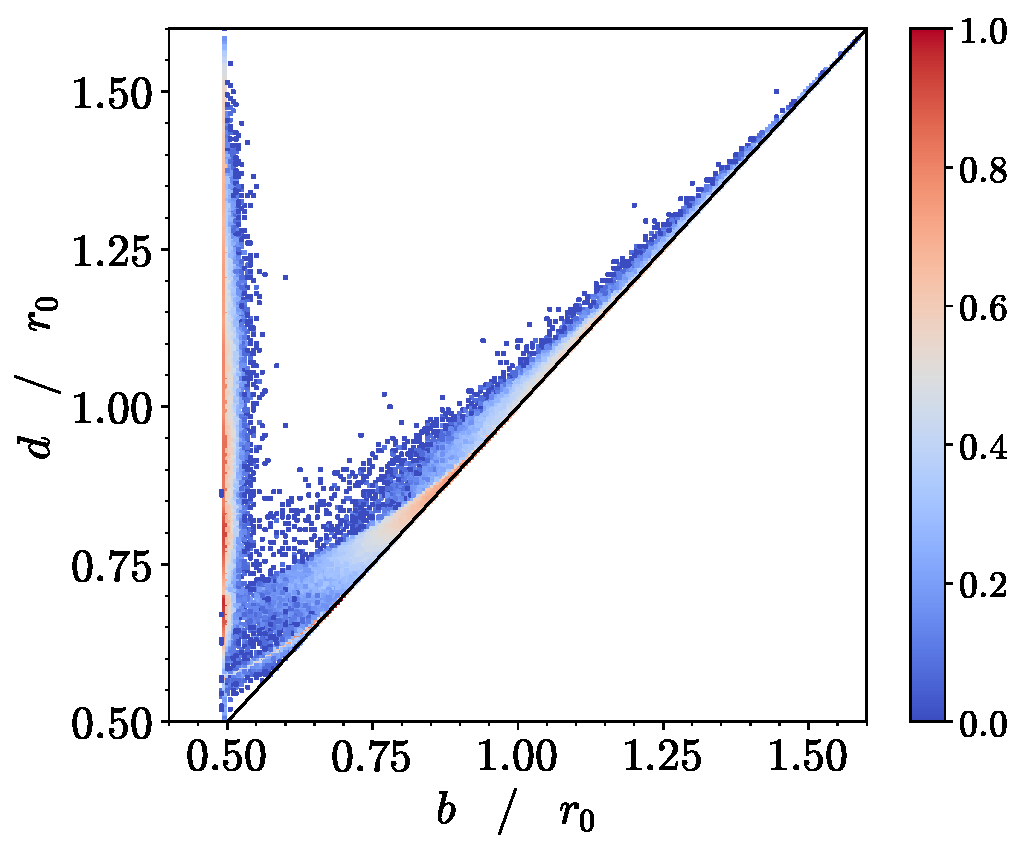
\includegraphics[width=\textwidth]{./figures/ph/t-1800_tr_pd.pdf}
         \caption{}
         \label{fig:trpdd}
     \end{subfigure}
     \hfill
    
	\caption{XXXX}
	\label{fig:}
\end{figure}




\begin{figure}[tb]
	\centering
     
      \begin{subfigure}[b]{0.45\textwidth}
         \centering
         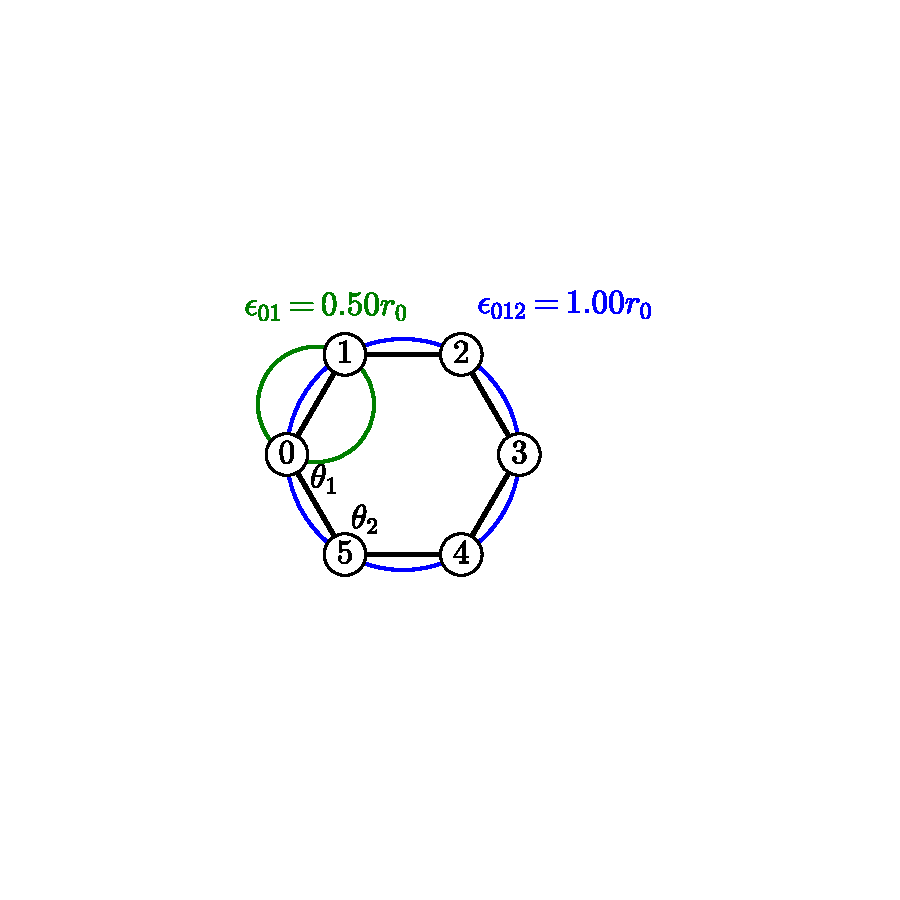
\includegraphics[width=0.75\textwidth]{./figures/ph/sl_hex_120.pdf}
         \caption{}
         \label{fig:slhex}
     \end{subfigure}
     
	 \vspace{0.5cm}     
     \begin{subfigure}[b]{0.45\textwidth}
         \centering
         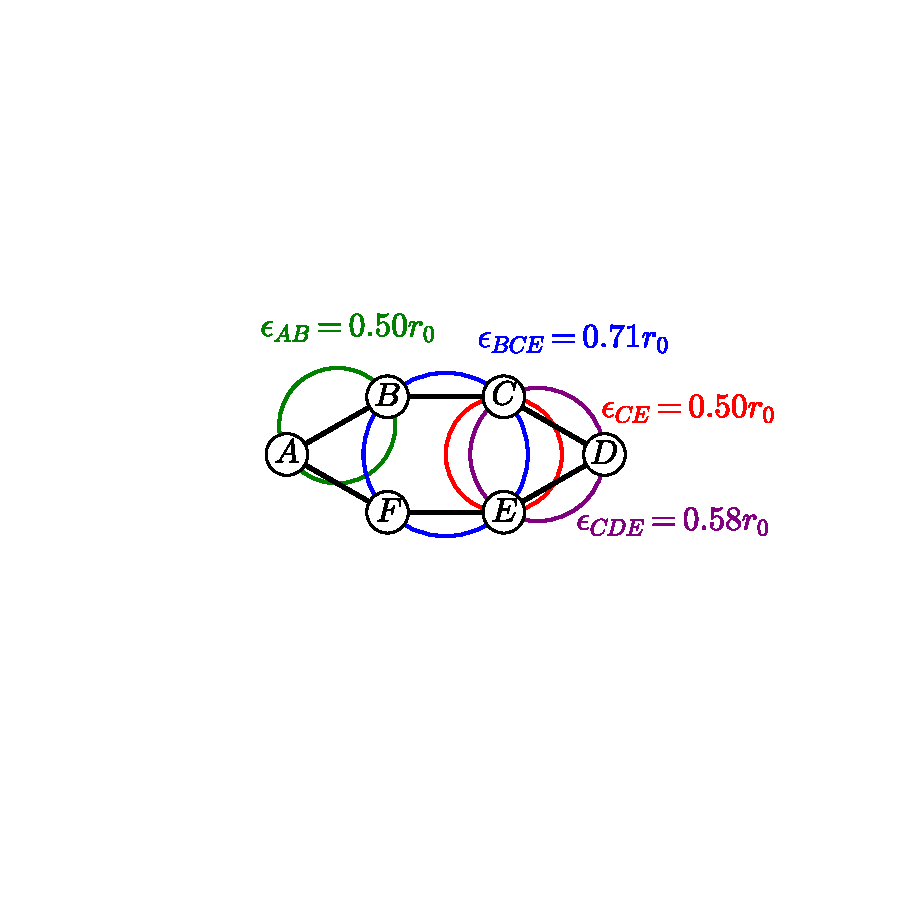
\includegraphics[width=0.9\textwidth]{./figures/ph/sl_hex_60.pdf}
         \caption{}
         \label{fig:slhex}
     \end{subfigure}
     \hfill
     \begin{subfigure}[b]{0.45\textwidth}
         \centering
         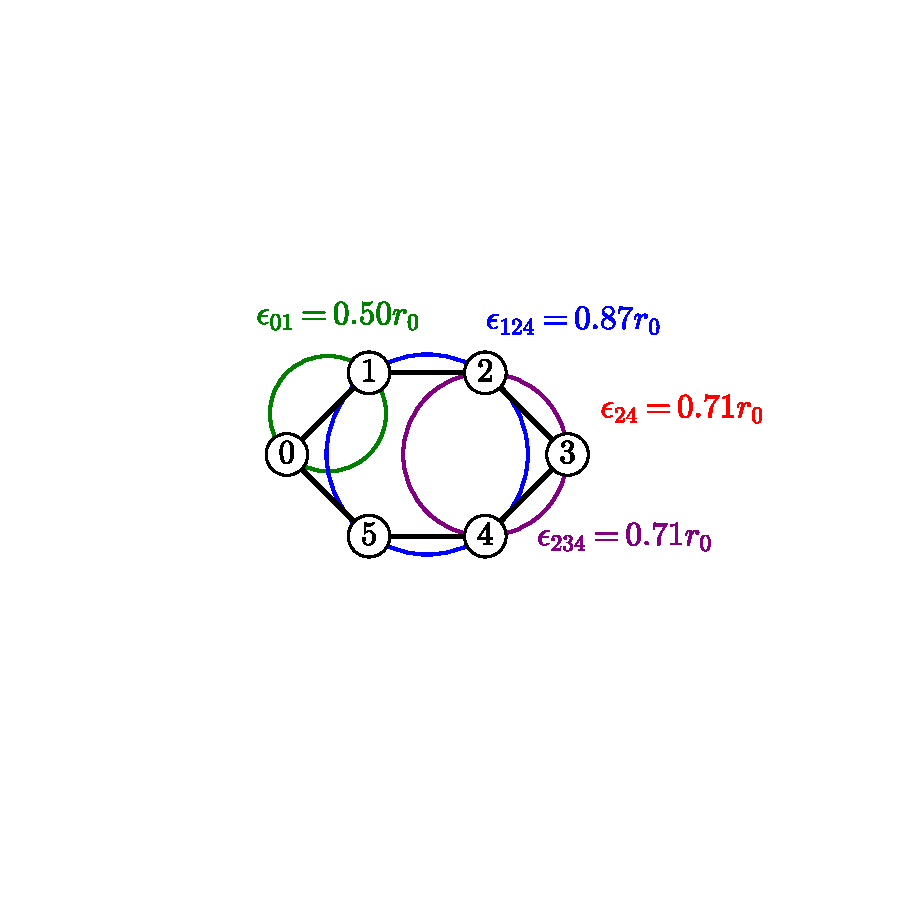
\includegraphics[width=0.9\textwidth]{./figures/ph/sl_hex_90.pdf}
         \caption{}
         \label{fig:slhex}
     \end{subfigure}
     
     \vspace{0.5cm}
     \begin{subfigure}[b]{0.45\textwidth}
         \centering
         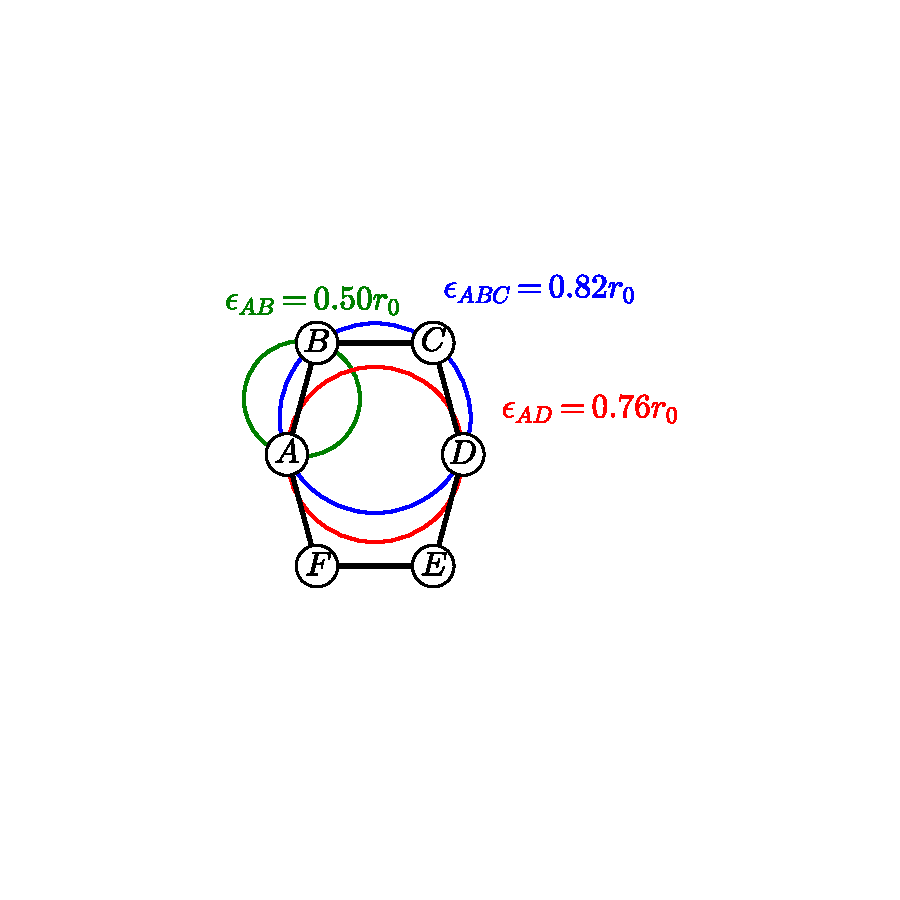
\includegraphics[width=0.8\textwidth]{./figures/ph/sl_hex_150.pdf}
         \caption{}
         \label{fig:slhex}
     \end{subfigure}
     \hfill
     \begin{subfigure}[b]{0.45\textwidth}
         \centering
         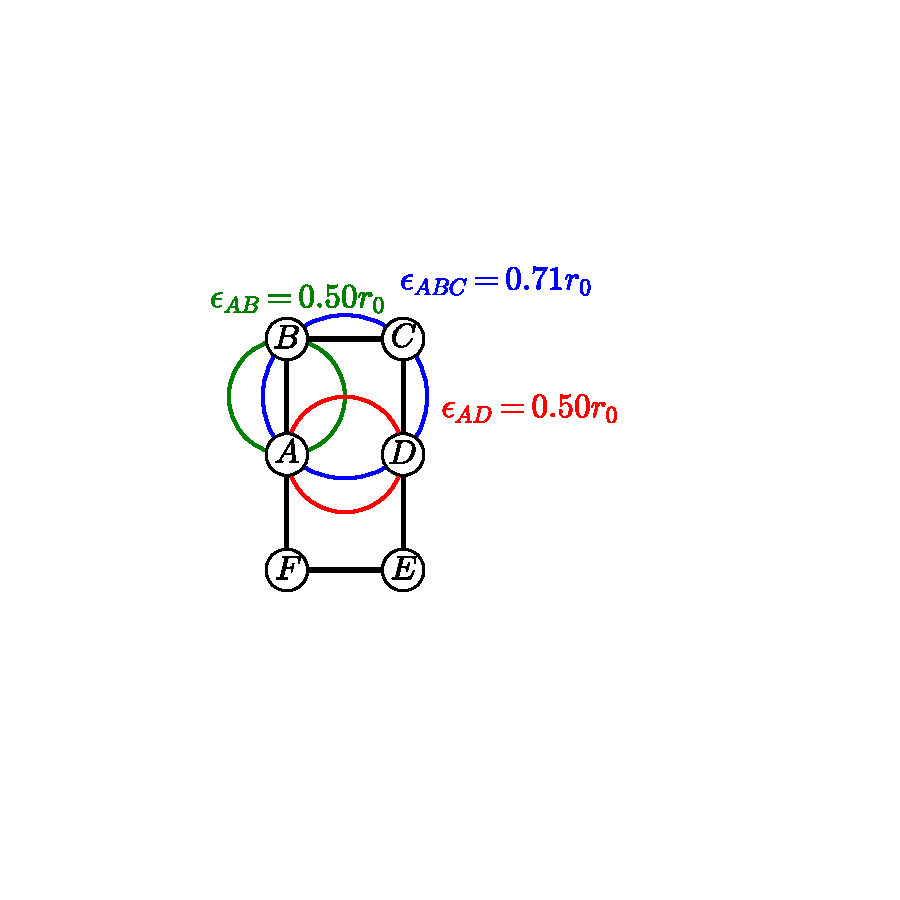
\includegraphics[width=0.7\textwidth]{./figures/ph/sl_hex_180.pdf}
         \caption{}
         \label{fig:slhex}
     \end{subfigure}
 
     
   
	\caption{XXXX}
	\label{fig:}
\end{figure}








\begin{figure}[tb]
	\centering
     
      \begin{subfigure}[b]{0.45\textwidth}
         \centering
         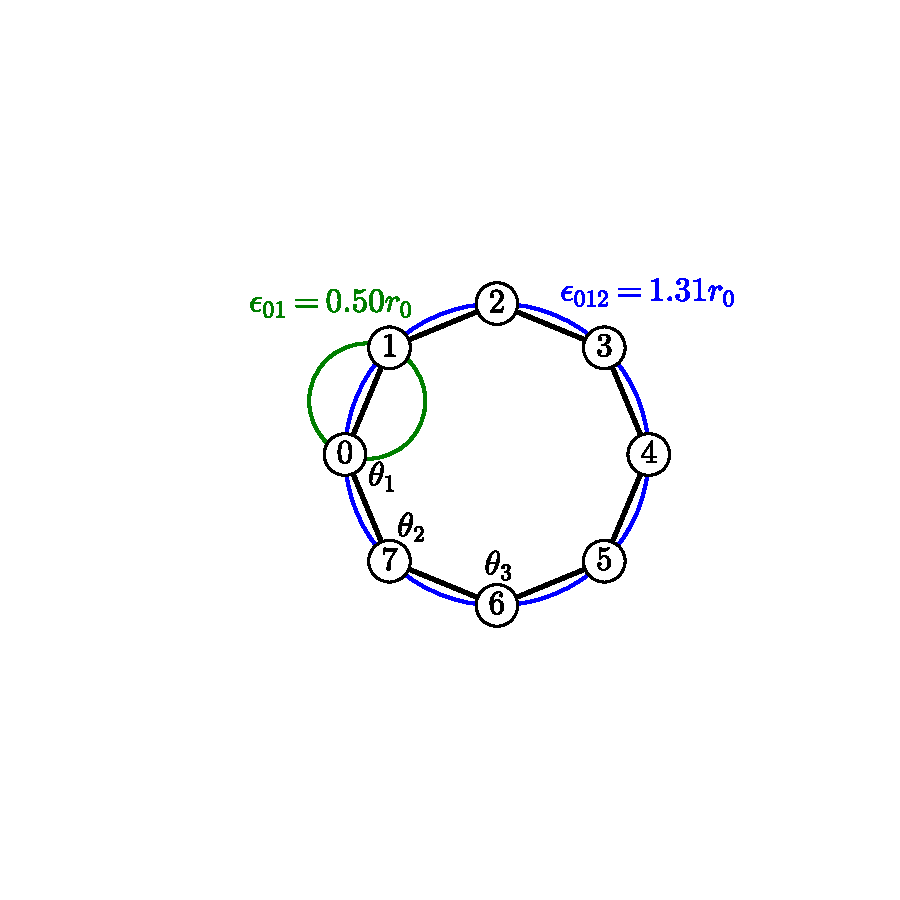
\includegraphics[width=0.85\textwidth]{./figures/ph/sl_oct_135.pdf}
         \caption{$\theta_1=134^\circ$, $\theta_2=135^\circ$, \\$\theta_3=136^\circ$}
         \label{fig:sloct}
     \end{subfigure}
     
     \vspace{0.5cm}
     \hfill
       \begin{subfigure}[b]{0.45\textwidth}
         \centering
         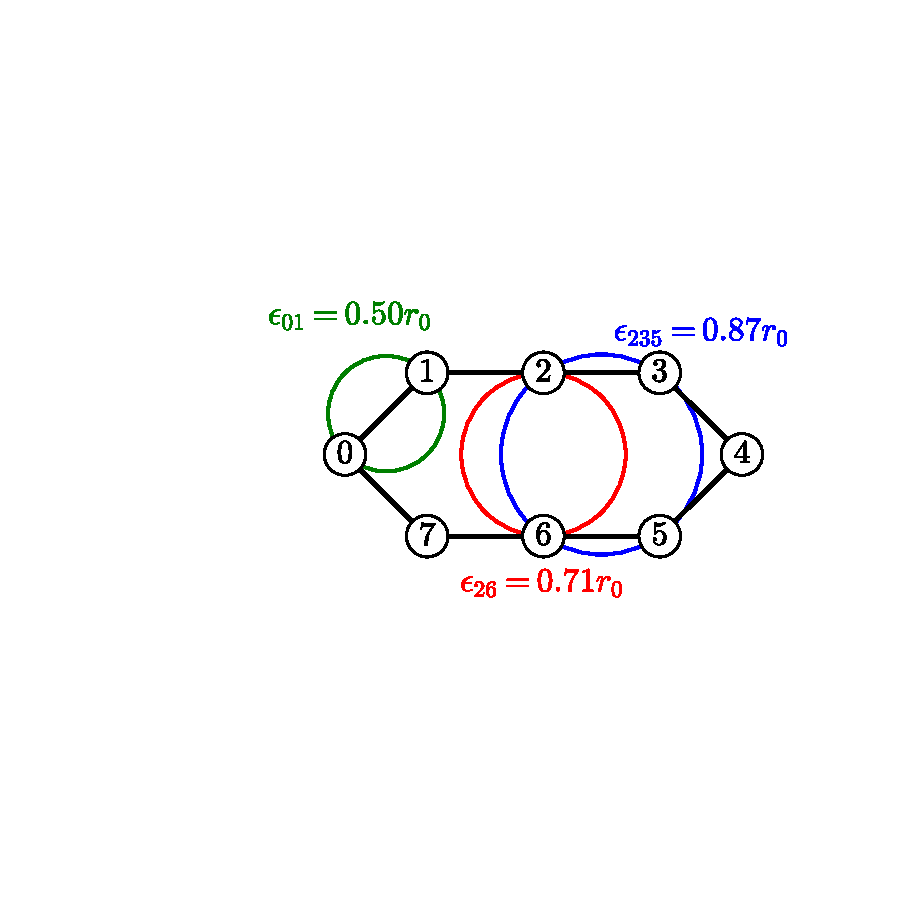
\includegraphics[width=0.95\textwidth]{./figures/ph/sl_oct_90.pdf}
         \caption{$\theta_1=112^\circ$, $\theta_2=135^\circ$, \\$\theta_3=158^\circ$}
         \label{fig:sloct}
     \end{subfigure}
     \hfill
       \begin{subfigure}[b]{0.45\textwidth}
         \centering
         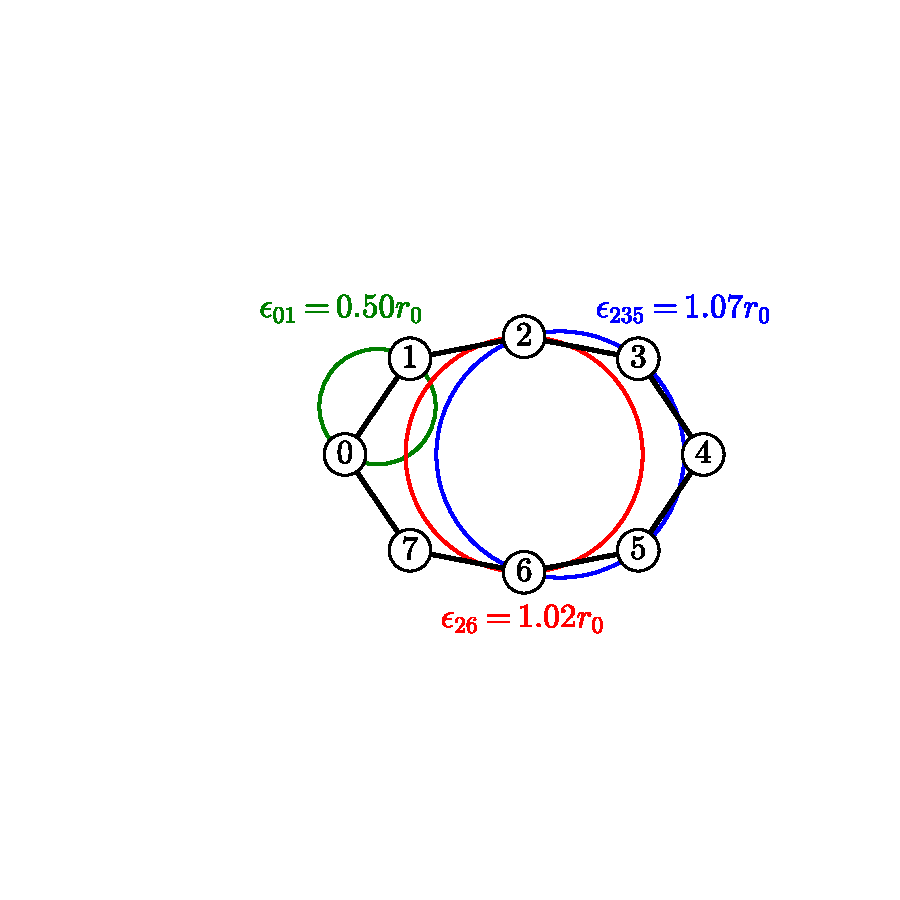
\includegraphics[width=0.85\textwidth]{./figures/ph/sl_oct_112.pdf}
         \caption{$\theta_1=90^\circ$, $\theta_2=135^\circ$, \\$\theta_3=180^\circ$}
         \label{fig:sloct}
     \end{subfigure}
     
     

	\caption{XXXX}
	\label{fig:}
\end{figure}

\begin{figure}[tb]
	\centering
     
      \begin{subfigure}[b]{0.45\textwidth}
         \centering
         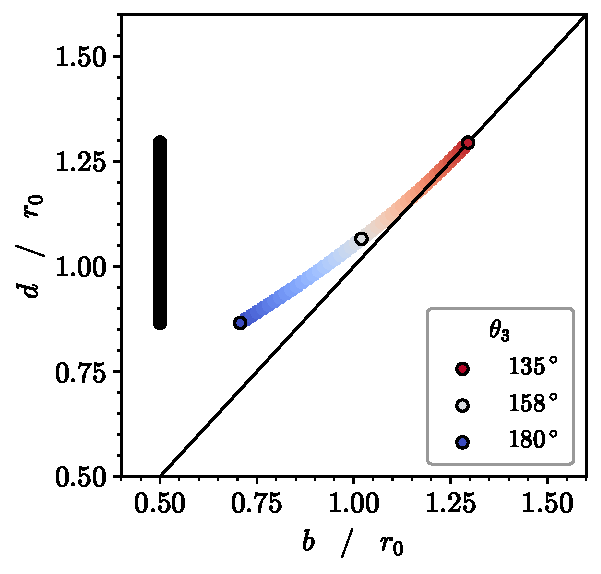
\includegraphics[width=\textwidth]{./figures/ph/sl_oct.pdf}
         \caption{}
         \label{fig:slx}
     \end{subfigure}
 
     
     

	\caption{XXXX}
	\label{fig:}
\end{figure}


\begin{figure}[tb]
	\centering
     
      \begin{subfigure}[b]{0.48\textwidth}
         \centering
         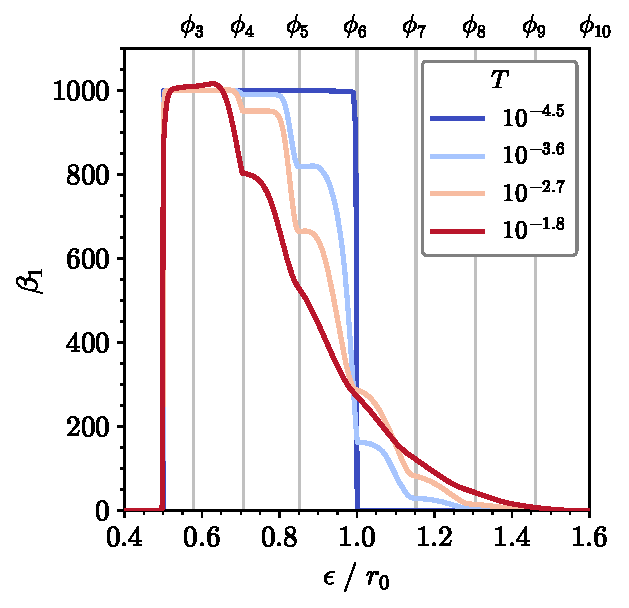
\includegraphics[width=\textwidth]{./figures/ph/tri_raft_beta1_full.pdf}
         \caption{}
         \label{fig:trpda}
     \end{subfigure}

	\caption{XXXX}
	\label{fig:}
\end{figure}

\begin{figure}[tb]
	\centering
     
      \begin{subfigure}[b]{0.48\textwidth}
         \centering
         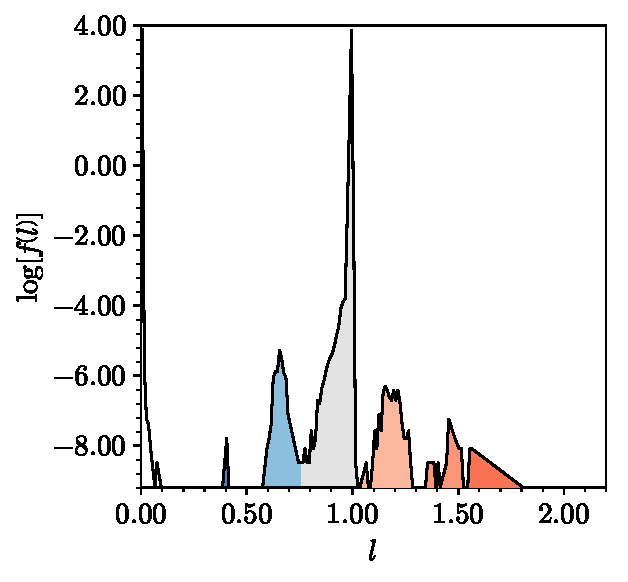
\includegraphics[width=\textwidth]{./figures/ph/tri_lt_dist_t-4500.pdf}
         \caption{}
         \label{fig:trpda}
     \end{subfigure}
     \hfill
      \begin{subfigure}[b]{0.48\textwidth}
         \centering
         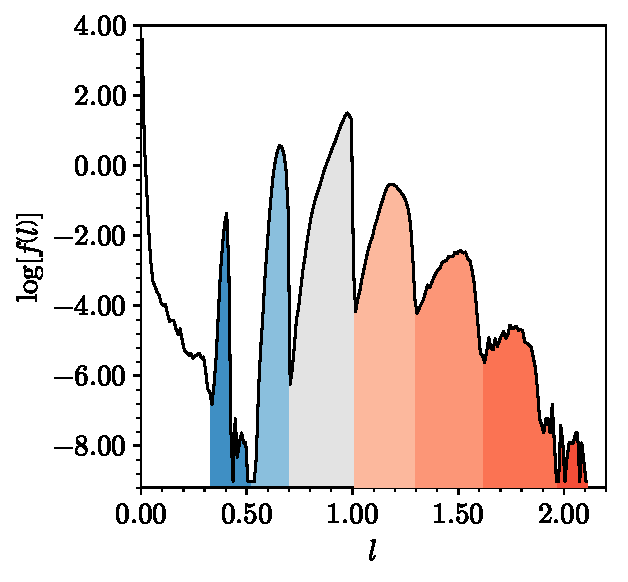
\includegraphics[width=\textwidth]{./figures/ph/tri_lt_dist_t-3600.pdf}
         \caption{}
         \label{fig:trpda}
     \end{subfigure}
     \hfill
     
     \begin{subfigure}[b]{0.48\textwidth}
         \centering
         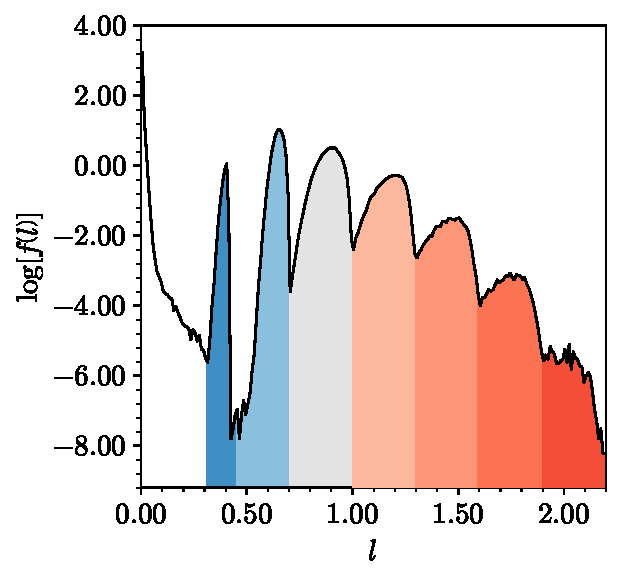
\includegraphics[width=\textwidth]{./figures/ph/tri_lt_dist_t-2700.pdf}
         \caption{}
         \label{fig:trpda}
     \end{subfigure}
     \hfill
      \begin{subfigure}[b]{0.48\textwidth}
         \centering
         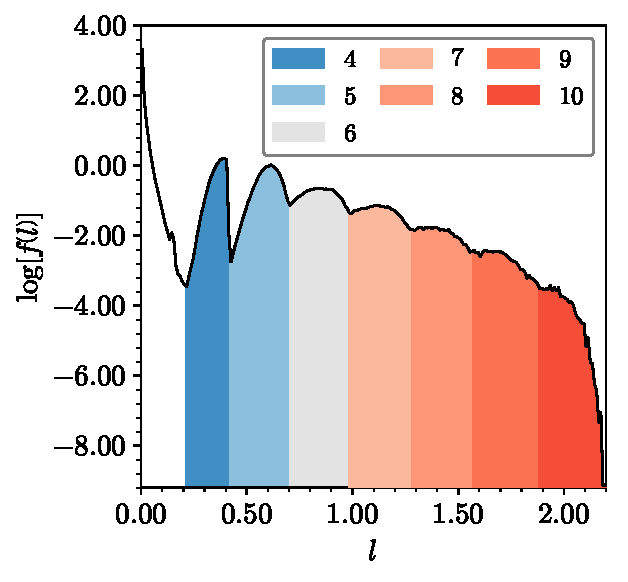
\includegraphics[width=\textwidth]{./figures/ph/tri_lt_dist_t-1800.pdf}
         \caption{}
         \label{fig:trpda}
     \end{subfigure}
     \hfill
    
	\caption{XXXX}
	\label{fig:}
\end{figure}

\section{Persistent Homology with CRNs}

\begin{figure}[tb]
	\centering
     
      \begin{subfigure}[b]{0.48\textwidth}
         \centering
         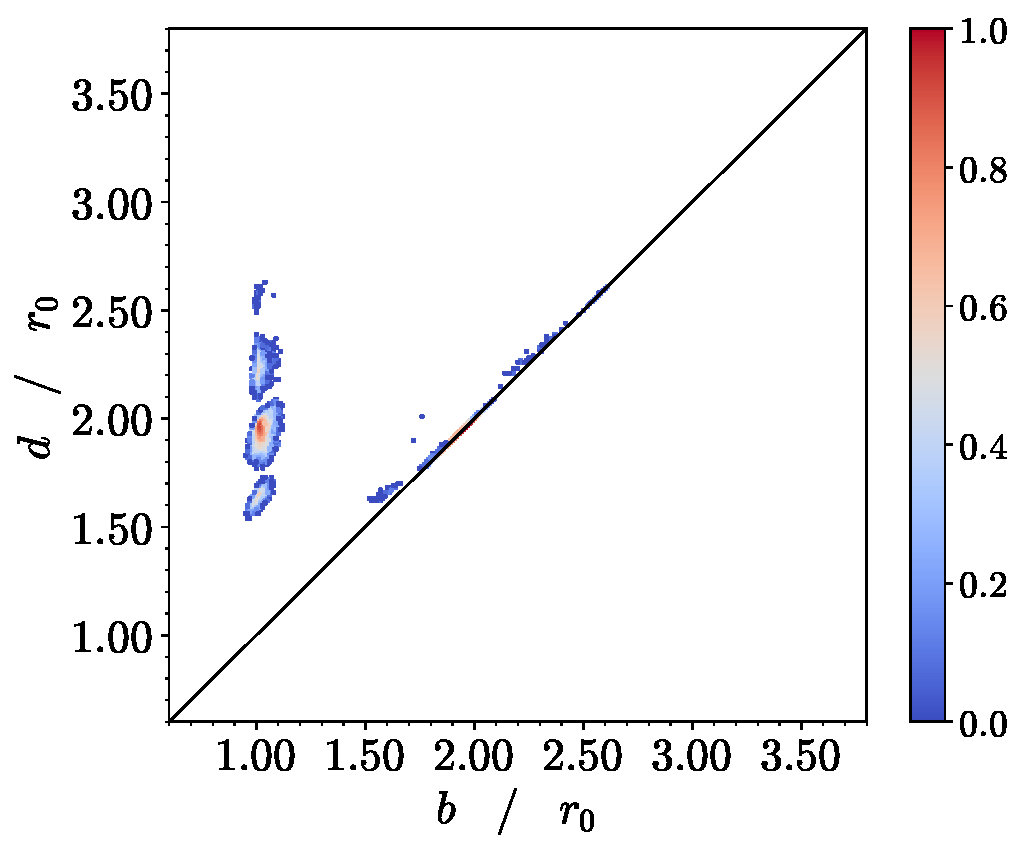
\includegraphics[width=\textwidth]{./figures/ph/t399_bs_pd.pdf}
         \caption{}
         \label{fig:trpda}
     \end{subfigure}
     \hfill
        \begin{subfigure}[b]{0.48\textwidth}
         \centering
         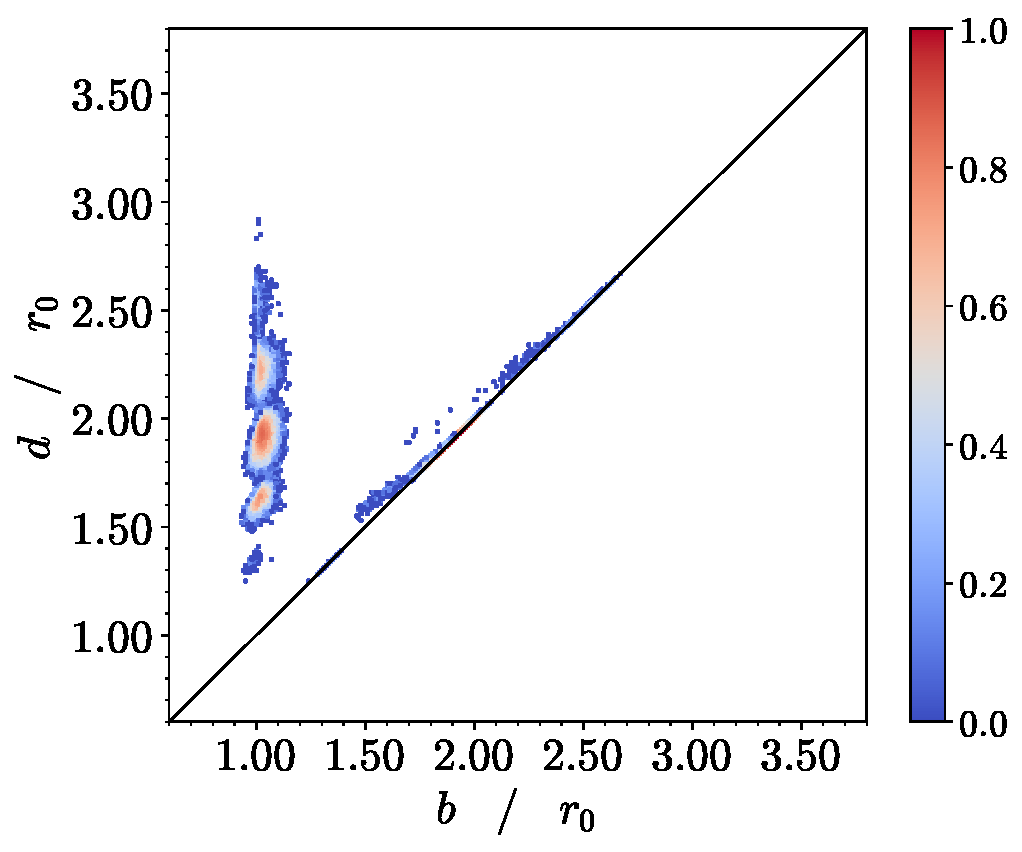
\includegraphics[width=\textwidth]{./figures/ph/t299_bs_pd.pdf}
         \caption{}
         \label{fig:trpda}
     \end{subfigure}
     \hfill
        \begin{subfigure}[b]{0.48\textwidth}
         \centering
         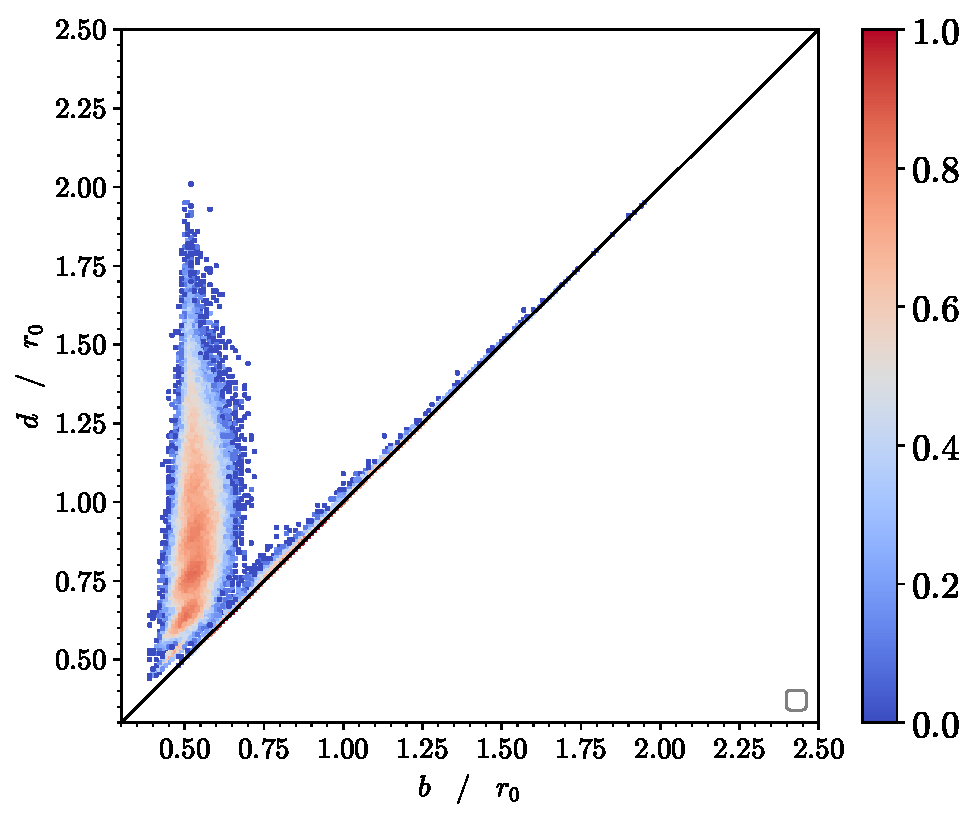
\includegraphics[width=\textwidth]{./figures/ph/t199_bs_pd.pdf}
         \caption{}
         \label{fig:trpda}
     \end{subfigure}
     \hfill
      \begin{subfigure}[b]{0.48\textwidth}
         \centering
         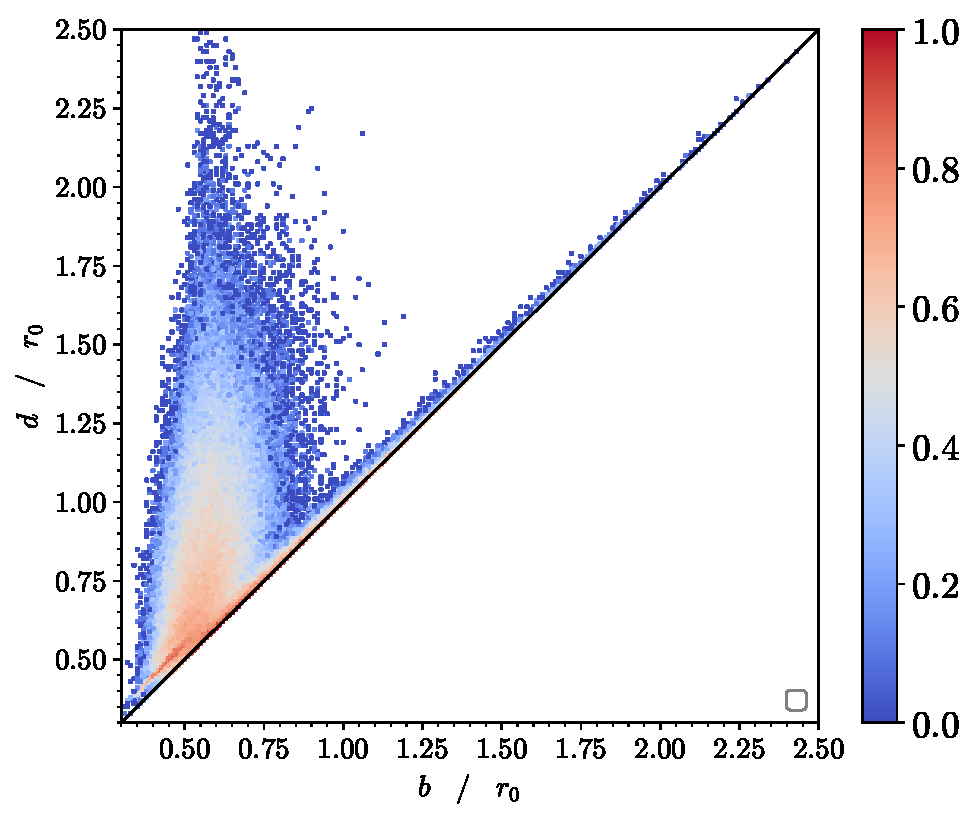
\includegraphics[width=\textwidth]{./figures/ph/t0_bs_pd.pdf}
         \caption{}
         \label{fig:trpda}
     \end{subfigure}

     
  
    
	\caption{XXXX}
	\label{fig:}
\end{figure}

\section{Chapter Summary}